\documentclass[]{article}
\usepackage{lmodern}
\usepackage{amssymb,amsmath}
\usepackage{ifxetex,ifluatex}
\usepackage{fixltx2e} % provides \textsubscript
\ifnum 0\ifxetex 1\fi\ifluatex 1\fi=0 % if pdftex
  \usepackage[T1]{fontenc}
  \usepackage[utf8]{inputenc}
\else % if luatex or xelatex
  \ifxetex
    \usepackage{mathspec}
  \else
    \usepackage{fontspec}
  \fi
  \defaultfontfeatures{Ligatures=TeX,Scale=MatchLowercase}
\fi
% use upquote if available, for straight quotes in verbatim environments
\IfFileExists{upquote.sty}{\usepackage{upquote}}{}
% use microtype if available
\IfFileExists{microtype.sty}{%
\usepackage{microtype}
\UseMicrotypeSet[protrusion]{basicmath} % disable protrusion for tt fonts
}{}
\usepackage[margin=1in]{geometry}
\usepackage{hyperref}
\hypersetup{unicode=true,
            pdftitle={hw1},
            pdfauthor={Zihao\_Wang},
            pdfborder={0 0 0},
            breaklinks=true}
\urlstyle{same}  % don't use monospace font for urls
\usepackage{color}
\usepackage{fancyvrb}
\newcommand{\VerbBar}{|}
\newcommand{\VERB}{\Verb[commandchars=\\\{\}]}
\DefineVerbatimEnvironment{Highlighting}{Verbatim}{commandchars=\\\{\}}
% Add ',fontsize=\small' for more characters per line
\usepackage{framed}
\definecolor{shadecolor}{RGB}{248,248,248}
\newenvironment{Shaded}{\begin{snugshade}}{\end{snugshade}}
\newcommand{\KeywordTok}[1]{\textcolor[rgb]{0.13,0.29,0.53}{\textbf{#1}}}
\newcommand{\DataTypeTok}[1]{\textcolor[rgb]{0.13,0.29,0.53}{#1}}
\newcommand{\DecValTok}[1]{\textcolor[rgb]{0.00,0.00,0.81}{#1}}
\newcommand{\BaseNTok}[1]{\textcolor[rgb]{0.00,0.00,0.81}{#1}}
\newcommand{\FloatTok}[1]{\textcolor[rgb]{0.00,0.00,0.81}{#1}}
\newcommand{\ConstantTok}[1]{\textcolor[rgb]{0.00,0.00,0.00}{#1}}
\newcommand{\CharTok}[1]{\textcolor[rgb]{0.31,0.60,0.02}{#1}}
\newcommand{\SpecialCharTok}[1]{\textcolor[rgb]{0.00,0.00,0.00}{#1}}
\newcommand{\StringTok}[1]{\textcolor[rgb]{0.31,0.60,0.02}{#1}}
\newcommand{\VerbatimStringTok}[1]{\textcolor[rgb]{0.31,0.60,0.02}{#1}}
\newcommand{\SpecialStringTok}[1]{\textcolor[rgb]{0.31,0.60,0.02}{#1}}
\newcommand{\ImportTok}[1]{#1}
\newcommand{\CommentTok}[1]{\textcolor[rgb]{0.56,0.35,0.01}{\textit{#1}}}
\newcommand{\DocumentationTok}[1]{\textcolor[rgb]{0.56,0.35,0.01}{\textbf{\textit{#1}}}}
\newcommand{\AnnotationTok}[1]{\textcolor[rgb]{0.56,0.35,0.01}{\textbf{\textit{#1}}}}
\newcommand{\CommentVarTok}[1]{\textcolor[rgb]{0.56,0.35,0.01}{\textbf{\textit{#1}}}}
\newcommand{\OtherTok}[1]{\textcolor[rgb]{0.56,0.35,0.01}{#1}}
\newcommand{\FunctionTok}[1]{\textcolor[rgb]{0.00,0.00,0.00}{#1}}
\newcommand{\VariableTok}[1]{\textcolor[rgb]{0.00,0.00,0.00}{#1}}
\newcommand{\ControlFlowTok}[1]{\textcolor[rgb]{0.13,0.29,0.53}{\textbf{#1}}}
\newcommand{\OperatorTok}[1]{\textcolor[rgb]{0.81,0.36,0.00}{\textbf{#1}}}
\newcommand{\BuiltInTok}[1]{#1}
\newcommand{\ExtensionTok}[1]{#1}
\newcommand{\PreprocessorTok}[1]{\textcolor[rgb]{0.56,0.35,0.01}{\textit{#1}}}
\newcommand{\AttributeTok}[1]{\textcolor[rgb]{0.77,0.63,0.00}{#1}}
\newcommand{\RegionMarkerTok}[1]{#1}
\newcommand{\InformationTok}[1]{\textcolor[rgb]{0.56,0.35,0.01}{\textbf{\textit{#1}}}}
\newcommand{\WarningTok}[1]{\textcolor[rgb]{0.56,0.35,0.01}{\textbf{\textit{#1}}}}
\newcommand{\AlertTok}[1]{\textcolor[rgb]{0.94,0.16,0.16}{#1}}
\newcommand{\ErrorTok}[1]{\textcolor[rgb]{0.64,0.00,0.00}{\textbf{#1}}}
\newcommand{\NormalTok}[1]{#1}
\usepackage{graphicx,grffile}
\makeatletter
\def\maxwidth{\ifdim\Gin@nat@width>\linewidth\linewidth\else\Gin@nat@width\fi}
\def\maxheight{\ifdim\Gin@nat@height>\textheight\textheight\else\Gin@nat@height\fi}
\makeatother
% Scale images if necessary, so that they will not overflow the page
% margins by default, and it is still possible to overwrite the defaults
% using explicit options in \includegraphics[width, height, ...]{}
\setkeys{Gin}{width=\maxwidth,height=\maxheight,keepaspectratio}
\IfFileExists{parskip.sty}{%
\usepackage{parskip}
}{% else
\setlength{\parindent}{0pt}
\setlength{\parskip}{6pt plus 2pt minus 1pt}
}
\setlength{\emergencystretch}{3em}  % prevent overfull lines
\providecommand{\tightlist}{%
  \setlength{\itemsep}{0pt}\setlength{\parskip}{0pt}}
\setcounter{secnumdepth}{0}
% Redefines (sub)paragraphs to behave more like sections
\ifx\paragraph\undefined\else
\let\oldparagraph\paragraph
\renewcommand{\paragraph}[1]{\oldparagraph{#1}\mbox{}}
\fi
\ifx\subparagraph\undefined\else
\let\oldsubparagraph\subparagraph
\renewcommand{\subparagraph}[1]{\oldsubparagraph{#1}\mbox{}}
\fi

%%% Use protect on footnotes to avoid problems with footnotes in titles
\let\rmarkdownfootnote\footnote%
\def\footnote{\protect\rmarkdownfootnote}

%%% Change title format to be more compact
\usepackage{titling}

% Create subtitle command for use in maketitle
\newcommand{\subtitle}[1]{
  \posttitle{
    \begin{center}\large#1\end{center}
    }
}

\setlength{\droptitle}{-2em}
  \title{hw1}
  \pretitle{\vspace{\droptitle}\centering\huge}
  \posttitle{\par}
  \author{Zihao\_Wang}
  \preauthor{\centering\large\emph}
  \postauthor{\par}
  \predate{\centering\large\emph}
  \postdate{\par}
  \date{10/7/2018}


\begin{document}
\maketitle

\begin{Shaded}
\begin{Highlighting}[]
\KeywordTok{rm}\NormalTok{(}\DataTypeTok{list=}\KeywordTok{ls}\NormalTok{())}
\KeywordTok{set.seed}\NormalTok{(}\DecValTok{12345}\NormalTok{)}
\KeywordTok{options}\NormalTok{(}\DataTypeTok{warn =} \OperatorTok{-}\DecValTok{1}\NormalTok{)}
\NormalTok{knitr}\OperatorTok{::}\NormalTok{opts_knit}\OperatorTok{$}\KeywordTok{set}\NormalTok{(}\DataTypeTok{root.dir =} \StringTok{'~/Desktop/stat374-fall-2018/analysis/'}\NormalTok{)}
\KeywordTok{library}\NormalTok{(kedd)}
\KeywordTok{library}\NormalTok{(locfit)}
\end{Highlighting}
\end{Shaded}

\begin{verbatim}
## locfit 1.5-9.1    2013-03-22
\end{verbatim}

\begin{Shaded}
\begin{Highlighting}[]
\KeywordTok{library}\NormalTok{(gridExtra)}
\KeywordTok{library}\NormalTok{(reshape)}
\KeywordTok{library}\NormalTok{(gam)}
\end{Highlighting}
\end{Shaded}

\begin{verbatim}
## Loading required package: splines
\end{verbatim}

\begin{verbatim}
## Loading required package: foreach
\end{verbatim}

\begin{verbatim}
## Loaded gam 1.16
\end{verbatim}

\begin{Shaded}
\begin{Highlighting}[]
\KeywordTok{library}\NormalTok{(tidyverse)}
\end{Highlighting}
\end{Shaded}

\begin{verbatim}
## -- Attaching packages ----------------------------------------------------------------------------------------------------------- tidyverse 1.2.1 --
\end{verbatim}

\begin{verbatim}
## √ ggplot2 2.2.1     √ purrr   0.2.5
## √ tibble  1.4.2     √ dplyr   0.7.4
## √ tidyr   0.8.1     √ stringr 1.3.1
## √ readr   1.1.1     √ forcats 0.3.0
\end{verbatim}

\begin{verbatim}
## -- Conflicts -------------------------------------------------------------------------------------------------------------- tidyverse_conflicts() --
## x purrr::accumulate() masks foreach::accumulate()
## x dplyr::combine()    masks gridExtra::combine()
## x tidyr::expand()     masks reshape::expand()
## x dplyr::filter()     masks stats::filter()
## x dplyr::lag()        masks stats::lag()
## x dplyr::rename()     masks reshape::rename()
## x purrr::when()       masks foreach::when()
\end{verbatim}

\section{1. Computing and plotting with
R}\label{computing-and-plotting-with-r}

\subsection{(a)}\label{a}

\begin{Shaded}
\begin{Highlighting}[]
\NormalTok{## function to compute empirical mean square error }
\NormalTok{mse <-}\StringTok{ }\ControlFlowTok{function}\NormalTok{(n,sigma)\{}
\NormalTok{  mysample =}\StringTok{ }\KeywordTok{rnorm}\NormalTok{(}\DataTypeTok{n =}\NormalTok{ n, }\DataTypeTok{sd =}\NormalTok{ sigma, }\DataTypeTok{mean =} \DecValTok{1}\NormalTok{)}
  \KeywordTok{return}\NormalTok{((}\KeywordTok{mean}\NormalTok{(mysample)}\OperatorTok{-}\DecValTok{1}\NormalTok{)}\OperatorTok{^}\DecValTok{2}\NormalTok{)}
\NormalTok{\}}

\NormalTok{emse <-}\StringTok{ }\ControlFlowTok{function}\NormalTok{(n,sigma,B)\{}
  \KeywordTok{return}\NormalTok{(}\KeywordTok{mean}\NormalTok{(}\KeywordTok{replicate}\NormalTok{(B,}\KeywordTok{mse}\NormalTok{(n,sigma))))}
\NormalTok{\}}

\NormalTok{## simulate and plot}
\NormalTok{sigma =}\StringTok{ }\DecValTok{1}
\NormalTok{B =}\StringTok{ }\DecValTok{100}

\NormalTok{ns =}\StringTok{ }\KeywordTok{seq}\NormalTok{(}\DecValTok{1}\NormalTok{,}\DecValTok{1000}\NormalTok{,}\DecValTok{5}\NormalTok{)}
\NormalTok{results =}\StringTok{ }\KeywordTok{replicate}\NormalTok{(}\KeywordTok{length}\NormalTok{(ns),}\DecValTok{0}\NormalTok{)}
\NormalTok{theory =}\StringTok{ }\KeywordTok{replicate}\NormalTok{(}\KeywordTok{length}\NormalTok{(ns),}\DecValTok{0}\NormalTok{)}

\ControlFlowTok{for}\NormalTok{(i }\ControlFlowTok{in} \DecValTok{1}\OperatorTok{:}\KeywordTok{length}\NormalTok{(ns))\{}
\NormalTok{  results[i] =}\StringTok{ }\KeywordTok{emse}\NormalTok{(ns[i],sigma,B)}
\NormalTok{  theory[i] =}\StringTok{ }\NormalTok{sigma}\OperatorTok{^}\DecValTok{2}\OperatorTok{/}\NormalTok{ns[i]}
\NormalTok{\}}

\KeywordTok{plot}\NormalTok{(}\KeywordTok{log}\NormalTok{(ns), }\KeywordTok{log}\NormalTok{(results), }\DataTypeTok{xlab =} \StringTok{"n"}\NormalTok{, }\DataTypeTok{ylab =} \StringTok{"mse"}\NormalTok{)}
\KeywordTok{lines}\NormalTok{(}\KeywordTok{log}\NormalTok{(ns),}\KeywordTok{log}\NormalTok{(theory), }\DataTypeTok{col =} \StringTok{"red"}\NormalTok{)}
\end{Highlighting}
\end{Shaded}

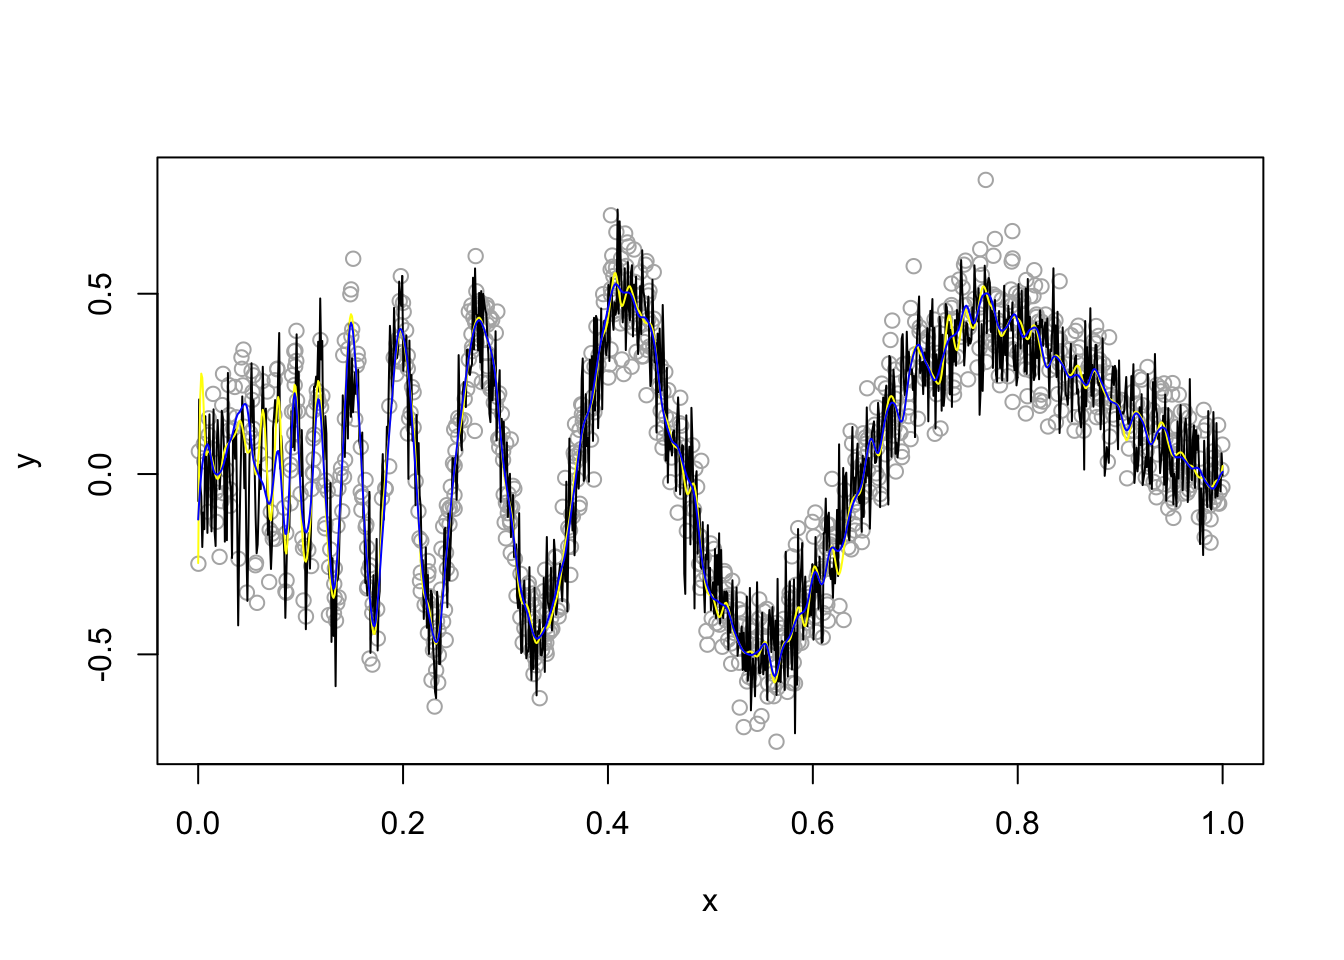
\includegraphics{hw1_files/figure-latex/unnamed-chunk-2-1.pdf}

\subsubsection{Comment:}\label{comment}

From the simulation experiments, we can see the results align with
theoretical results

\subsection{(b)}\label{b}

\begin{Shaded}
\begin{Highlighting}[]
\NormalTok{n =}\StringTok{ }\DecValTok{1000}
\NormalTok{sigma =}\StringTok{ }\DecValTok{1}
\NormalTok{B =}\StringTok{ }\DecValTok{10000}

\NormalTok{## simulation}
\NormalTok{Z =}\StringTok{ }\KeywordTok{replicate}\NormalTok{(B,}\KeywordTok{sqrt}\NormalTok{(n)}\OperatorTok{*}\NormalTok{(}\KeywordTok{mean}\NormalTok{(}\KeywordTok{rnorm}\NormalTok{(n,}\DecValTok{1}\NormalTok{,sigma)) }\OperatorTok{-}\StringTok{ }\DecValTok{1}\NormalTok{))}

\NormalTok{## theoretical standard normal}
\NormalTok{ns =}\StringTok{ }\KeywordTok{seq}\NormalTok{(}\OperatorTok{-}\DecValTok{10}\NormalTok{,}\DecValTok{10}\NormalTok{,}\FloatTok{0.01}\NormalTok{)}
\NormalTok{theory =}\StringTok{ }\KeywordTok{replicate}\NormalTok{(}\KeywordTok{length}\NormalTok{(ns),}\DecValTok{0}\NormalTok{)}
\ControlFlowTok{for}\NormalTok{(i }\ControlFlowTok{in} \DecValTok{1}\OperatorTok{:}\KeywordTok{length}\NormalTok{(ns))\{}
\NormalTok{  theory[i] =}\StringTok{ }\DecValTok{1}\OperatorTok{/}\KeywordTok{sqrt}\NormalTok{(}\DecValTok{2}\OperatorTok{*}\NormalTok{pi) }\OperatorTok{*}\StringTok{ }\KeywordTok{exp}\NormalTok{(}\OperatorTok{-}\NormalTok{ns[i]}\OperatorTok{^}\DecValTok{2} \OperatorTok{*}\FloatTok{0.5}\NormalTok{)}
\NormalTok{\}}

\KeywordTok{plot}\NormalTok{(}\KeywordTok{density}\NormalTok{(Z), }\DataTypeTok{col =} \StringTok{"blue"}\NormalTok{)}
\KeywordTok{lines}\NormalTok{(ns,theory,}\DataTypeTok{col =} \StringTok{"red"}\NormalTok{)}
\end{Highlighting}
\end{Shaded}

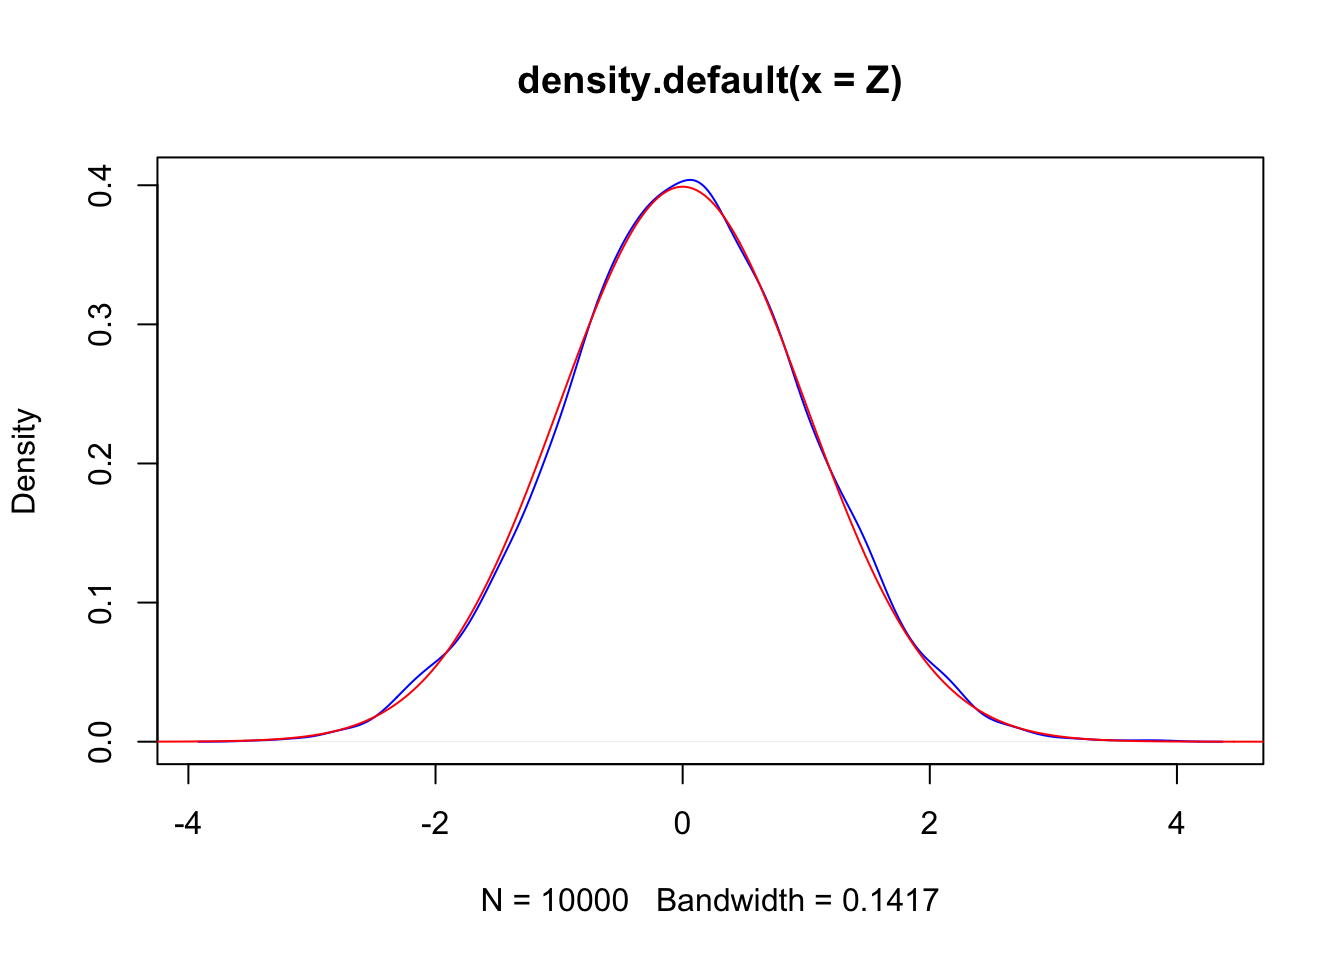
\includegraphics{hw1_files/figure-latex/unnamed-chunk-3-1.pdf} \#\#\#
Comment: When B is too small (say, only 100), \textbf{density(B)} does
not give very good estimate. When B is big enough, density estimation is
quite good.

\section{2 Leave-oue-out
cross-validation}\label{leave-oue-out-cross-validation}

\subsection{(a)}\label{a-1}

By definition,
\(\hat{R}(h) = \frac{1}{n} * \sum_{i = 1}^{n} (r(x_{i})-\hat{r}_{-i}(x_{i}))^2\).
Then we have
\(r(x_{i}) - \hat{r}_{-i}(x_{i}) = Y_{i} - \frac{\sum_{k \neq i} L_{i,k} * Y_{k}}{1-L_{ii}} = \frac{Y_{i} - \hat{r}_{n}(x_{i})} {1-L _{ii}}\).
Then our desired equation follows.

\subsection{(b)}\label{b-1}

Note: I select bandwidth in two ways: coding the loocv(bandwidth)
function myself, and using the gcv function in the package. The two
results are quite different, so I show both of them.

\subsubsection{See what the data looks
like}\label{see-what-the-data-looks-like}

\begin{Shaded}
\begin{Highlighting}[]
\NormalTok{Doppler <-}\StringTok{ }\ControlFlowTok{function}\NormalTok{(x)\{}
\NormalTok{  y =}\StringTok{ }\KeywordTok{sqrt}\NormalTok{(x}\OperatorTok{*}\NormalTok{(}\DecValTok{1}\OperatorTok{-}\NormalTok{x)) }\OperatorTok{*}\StringTok{ }\KeywordTok{sin}\NormalTok{(}\FloatTok{2.1}\OperatorTok{*}\NormalTok{pi}\OperatorTok{/}\NormalTok{(x}\OperatorTok{+}\FloatTok{0.05}\NormalTok{)) }
  \KeywordTok{return}\NormalTok{(y)}
\NormalTok{\}}

\NormalTok{N =}\StringTok{ }\DecValTok{1000}
\NormalTok{sigma =}\StringTok{ }\FloatTok{0.1}
\NormalTok{Xs =}\StringTok{ }\KeywordTok{seq}\NormalTok{(}\DecValTok{0}\NormalTok{,}\DecValTok{1}\NormalTok{, }\DataTypeTok{length =}\NormalTok{ N)}
\NormalTok{ys_true =}\StringTok{ }\KeywordTok{Doppler}\NormalTok{(Xs)}
\NormalTok{ys =}\StringTok{ }\NormalTok{ys_true }\OperatorTok{+}\StringTok{ }\KeywordTok{rnorm}\NormalTok{(N,}\DataTypeTok{sd =}\NormalTok{ sigma)}
\KeywordTok{plot}\NormalTok{(Xs,ys)}
\KeywordTok{lines}\NormalTok{(Xs,ys_true, }\DataTypeTok{col =} \StringTok{"red"}\NormalTok{)}
\end{Highlighting}
\end{Shaded}

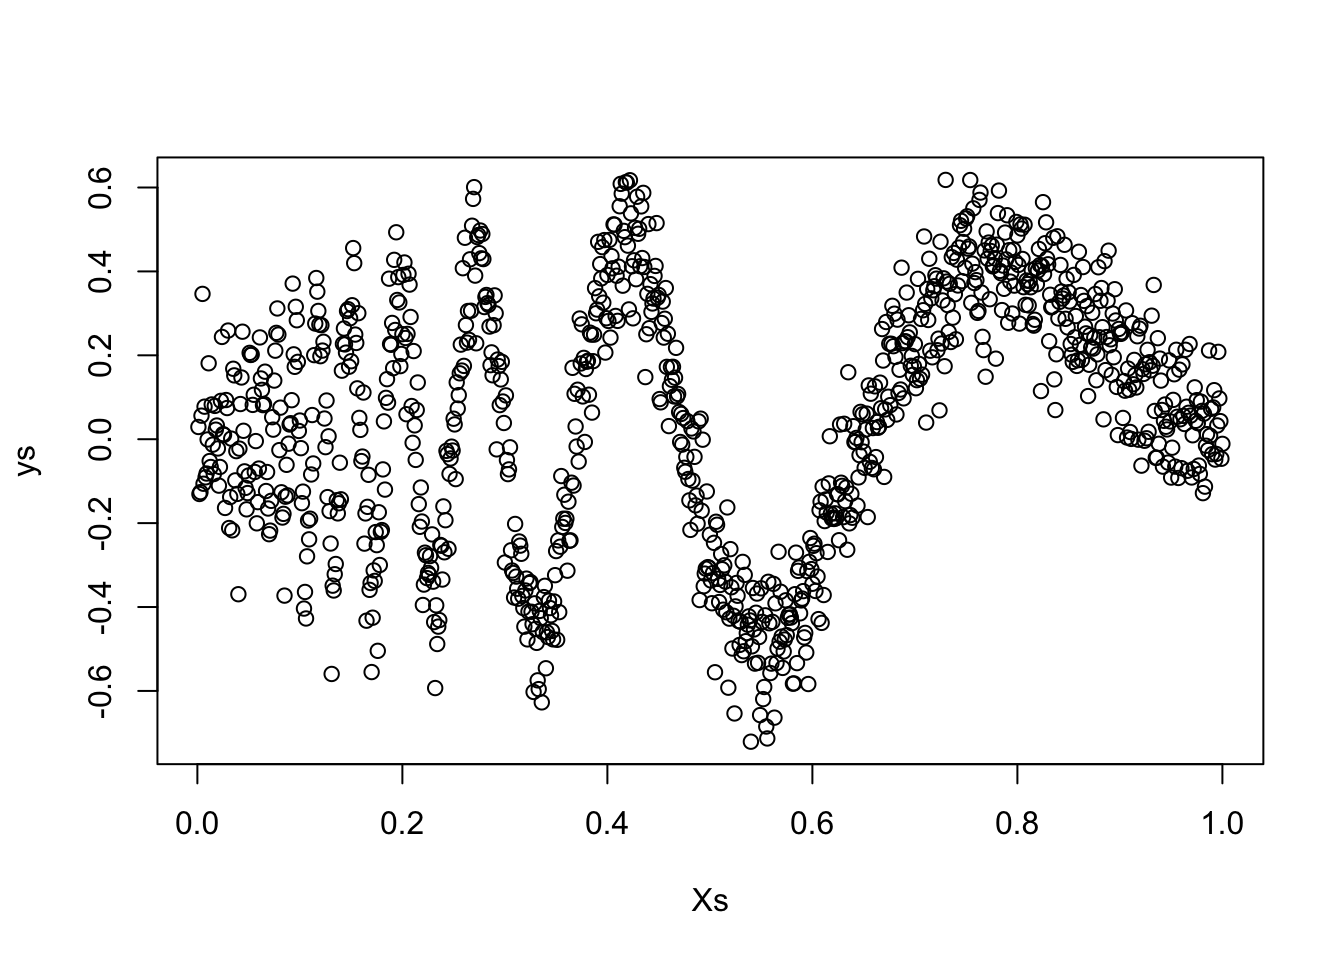
\includegraphics{hw1_files/figure-latex/unnamed-chunk-4-1.pdf}

\subsubsection{Plot Cross-validation-score vs
bandwidth}\label{plot-cross-validation-score-vs-bandwidth}

\begin{Shaded}
\begin{Highlighting}[]
\NormalTok{K <-}\StringTok{ }\ControlFlowTok{function}\NormalTok{(x)\{}
  \KeywordTok{return}\NormalTok{(}\DecValTok{1}\OperatorTok{/}\KeywordTok{sqrt}\NormalTok{(}\DecValTok{2}\OperatorTok{*}\NormalTok{pi) }\OperatorTok{*}\StringTok{ }\KeywordTok{exp}\NormalTok{(}\OperatorTok{-}\NormalTok{x}\OperatorTok{^}\DecValTok{2}\OperatorTok{/}\DecValTok{2}\NormalTok{))}
\NormalTok{\}}

\NormalTok{Rhat <-}\StringTok{ }\ControlFlowTok{function}\NormalTok{(h,Xs)\{}
\NormalTok{  ### compute L (L_ij = l_j(x_i), rowSums(L) = 1,1...)}
\NormalTok{  n =}\StringTok{ }\KeywordTok{length}\NormalTok{(Xs)}
\NormalTok{  X_matrix =}\StringTok{ }\KeywordTok{replicate}\NormalTok{(n,Xs)}
\NormalTok{  X_difference_scaled =}\StringTok{ }\NormalTok{(X_matrix }\OperatorTok{-}\StringTok{ }\KeywordTok{t}\NormalTok{(X_matrix))}\OperatorTok{/}\NormalTok{h }
\NormalTok{  X_difference_scaled_kernel =}\StringTok{ }\KeywordTok{K}\NormalTok{(X_difference_scaled) ## X_ij = K((Xi-Xj)/h)}
\NormalTok{  L =}\StringTok{ }\KeywordTok{diag}\NormalTok{(}\DecValTok{1}\OperatorTok{/}\KeywordTok{rowSums}\NormalTok{(X_difference_scaled_kernel)) }\OperatorTok\StringTok{ }\NormalTok{X_difference_scaled_kernel }
  
\NormalTok{  ### Compute Lii}
\NormalTok{  L_diag =}\StringTok{ }\KeywordTok{diag}\NormalTok{(L)}
  
\NormalTok{  ### Compute ys_hat}
\NormalTok{  ys_hat =}\StringTok{ }\NormalTok{L }\OperatorTok\StringTok{ }\NormalTok{ys}
  
\NormalTok{  ### Conmpute R_hat}
\NormalTok{  R_hat =}\StringTok{ }\KeywordTok{mean}\NormalTok{(((ys}\OperatorTok{-}\NormalTok{ys_hat)}\OperatorTok{/}\NormalTok{(}\DecValTok{1}\OperatorTok{-}\NormalTok{L_diag))}\OperatorTok{^}\DecValTok{2}\NormalTok{)}
  
  \KeywordTok{return}\NormalTok{(R_hat)}
\NormalTok{\}}
\end{Highlighting}
\end{Shaded}

\begin{Shaded}
\begin{Highlighting}[]
\NormalTok{hs =}\StringTok{ }\KeywordTok{seq}\NormalTok{(}\DecValTok{0}\NormalTok{,}\FloatTok{0.05}\NormalTok{,}\FloatTok{0.001}\NormalTok{)}
\NormalTok{myloocvs <-}\StringTok{ }\KeywordTok{readRDS}\NormalTok{(}\StringTok{"../data/loocvs_hw1_p2"}\NormalTok{) ## I save the computed results as it will take some time}
\CommentTok{#myloocvs <- sapply(hs, function(h) Rhat(h,Xs)) }
\KeywordTok{plot}\NormalTok{(myloocvs)}
\end{Highlighting}
\end{Shaded}

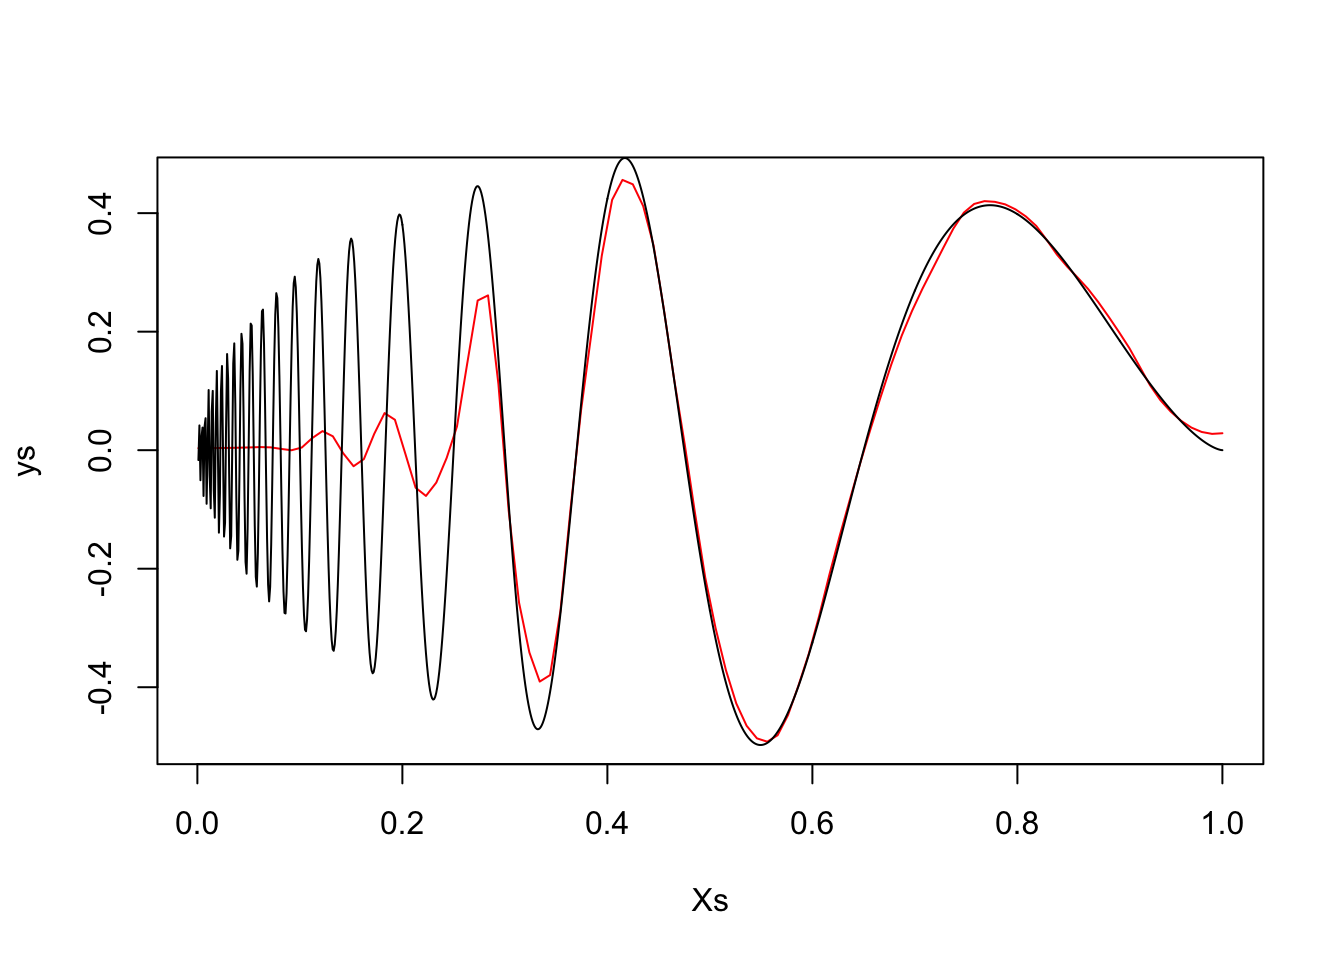
\includegraphics{hw1_files/figure-latex/unnamed-chunk-6-1.pdf}

\begin{Shaded}
\begin{Highlighting}[]
\CommentTok{#saveRDS(myloocvs,"../data/loocvs_hw1_p2.rds")}
\NormalTok{## We can also find the best bandwidth using gcv function, as an approximate (however, it gives me quite different results)}
\CommentTok{# gcvs = gcvplot(ys~Xs, alpha = seq(0,0.5,0.01))}
\CommentTok{# plot(gcvs$alpha, gcvs$values)}
\end{Highlighting}
\end{Shaded}

\subsubsection{locfit using the optimal
bandwidth}\label{locfit-using-the-optimal-bandwidth}

\begin{Shaded}
\begin{Highlighting}[]
\NormalTok{h_star =}\StringTok{ }\NormalTok{hs[}\KeywordTok{which.min}\NormalTok{(myloocvs)]}
\CommentTok{#h_star = 0.02}
\NormalTok{locfitopt =}\StringTok{ }\KeywordTok{locfit}\NormalTok{(ys}\OperatorTok{~}\NormalTok{Xs,}\DataTypeTok{alpha =}\NormalTok{ h_star) ## if the first the element is 0, it reports error! How does this affect estimation??}
\KeywordTok{plot}\NormalTok{(Xs, ys)}
\KeywordTok{lines}\NormalTok{(Xs,}\KeywordTok{predict}\NormalTok{(locfitopt, }\DataTypeTok{newdata =}\NormalTok{ Xs), }\DataTypeTok{type =} \StringTok{"l"}\NormalTok{,}\DataTypeTok{col =} \StringTok{"red"}\NormalTok{)}
\end{Highlighting}
\end{Shaded}

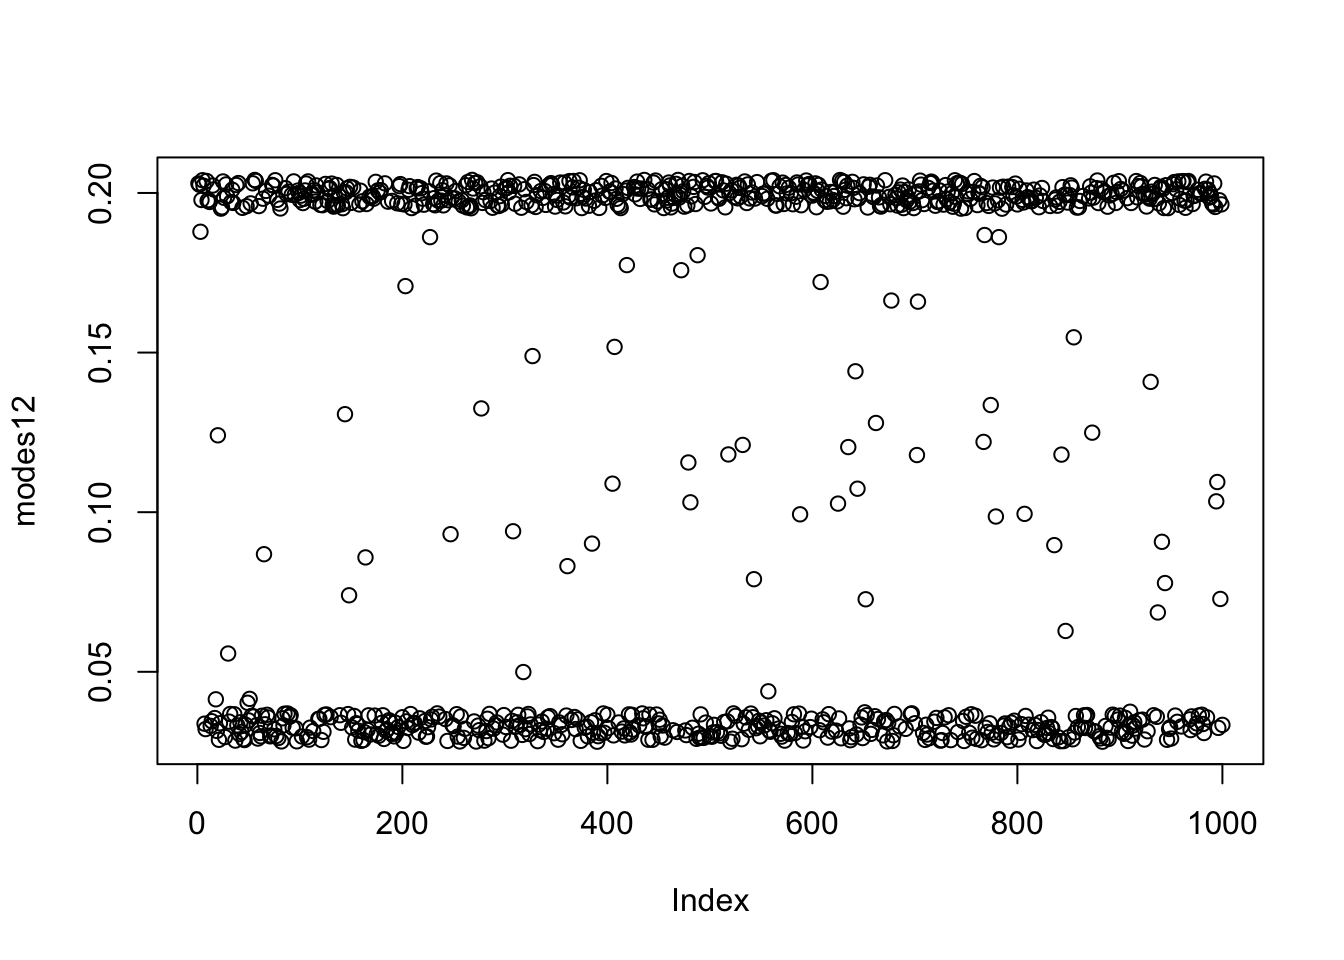
\includegraphics{hw1_files/figure-latex/unnamed-chunk-7-1.pdf}

\begin{Shaded}
\begin{Highlighting}[]
\CommentTok{#lines(xg, Doppler(xg), col = "blue")}
\end{Highlighting}
\end{Shaded}

\subsubsection{Comment:}\label{comment-1}

This should be the optimal, but from the plot it seems to be
undersmoothing a lot (especially compared with the results using gcv,
which will be shown later)

\subsection{compute and plot the confidence interval for
r(x)}\label{compute-and-plot-the-confidence-interval-for-rx}

\begin{Shaded}
\begin{Highlighting}[]
\NormalTok{## Formula: rhat(x) +- Z_a/2 * sigmahat(x) * |l(x)|}
\NormalTok{## Assumption: homoscedasticity of variance}
\NormalTok{## Formula for sigamhat(x): sigmahat(x) = sum(residue^2) / (n - 2*nu - 2*nutilde), where nu = tr(L), nutilde = tr(L^t*T)}
\NormalTok{## they can be retrived in dp1, dp2 respectively}

\NormalTok{nu =}\StringTok{ }\NormalTok{locfitopt}\OperatorTok{$}\NormalTok{dp[[}\StringTok{"df1"}\NormalTok{]]}
\NormalTok{nutilde =}\StringTok{ }\NormalTok{locfitopt}\OperatorTok{$}\NormalTok{dp[[}\StringTok{"df2"}\NormalTok{]]}
\NormalTok{sigmahat_sqrt =}\StringTok{ }\KeywordTok{sum}\NormalTok{(}\KeywordTok{residuals}\NormalTok{(locfitopt)}\OperatorTok{^}\DecValTok{2}\NormalTok{)}\OperatorTok{/}\NormalTok{(N }\OperatorTok{-}\StringTok{ }\DecValTok{2}\OperatorTok{*}\NormalTok{nu }\OperatorTok{+}\StringTok{ }\NormalTok{nutilde)}

\NormalTok{diaghat =}\StringTok{ }\KeywordTok{predict}\NormalTok{(locfitopt,}\DataTypeTok{where=}\StringTok{"data"}\NormalTok{,}\DataTypeTok{what=}\StringTok{"infl"}\NormalTok{) ## L_ii}
\NormalTok{normell =}\StringTok{ }\KeywordTok{predict}\NormalTok{(locfitopt,}\DataTypeTok{where=}\StringTok{"data"}\NormalTok{,}\DataTypeTok{what=}\StringTok{"vari"}\NormalTok{) ## |l_i(x)|}

\NormalTok{critval =}\StringTok{ }\FloatTok{1.96}
\NormalTok{xg =}\StringTok{ }\NormalTok{Xs}
\NormalTok{pred =}\StringTok{ }\KeywordTok{predict}\NormalTok{(locfitopt, }\DataTypeTok{newdata =}\NormalTok{ xg)}

\NormalTok{width =}\StringTok{ }\NormalTok{critval }\OperatorTok{*}\StringTok{ }\KeywordTok{sqrt}\NormalTok{(sigmahat_sqrt}\OperatorTok{*}\NormalTok{normell)}
\NormalTok{upper =}\StringTok{ }\NormalTok{pred }\OperatorTok{+}\StringTok{ }\NormalTok{width}
\NormalTok{lower =}\StringTok{ }\NormalTok{pred }\OperatorTok{-}\StringTok{ }\NormalTok{width}


\NormalTok{## plot confidence band}
\KeywordTok{plot}\NormalTok{(xg, pred,}\DataTypeTok{lwd=}\DecValTok{3}\NormalTok{, }\DataTypeTok{xlab=}\StringTok{"l"}\NormalTok{,}\DataTypeTok{ylab=}\StringTok{"Cl"}\NormalTok{,}\DataTypeTok{cex=}\DecValTok{3}\NormalTok{,}\DataTypeTok{cex.axis=}\FloatTok{1.3}\NormalTok{, }\DataTypeTok{cex.lab=}\FloatTok{1.3}\NormalTok{,}\DataTypeTok{type=}\StringTok{"l"}\NormalTok{)}
\KeywordTok{lines}\NormalTok{(xg, upper,}\DataTypeTok{col =} \DecValTok{2}\NormalTok{, }\DataTypeTok{lwd =} \DecValTok{3}\NormalTok{)}
\KeywordTok{lines}\NormalTok{(xg, lower,}\DataTypeTok{col =} \DecValTok{3}\NormalTok{, }\DataTypeTok{lwd =} \DecValTok{2}\NormalTok{)}
\end{Highlighting}
\end{Shaded}

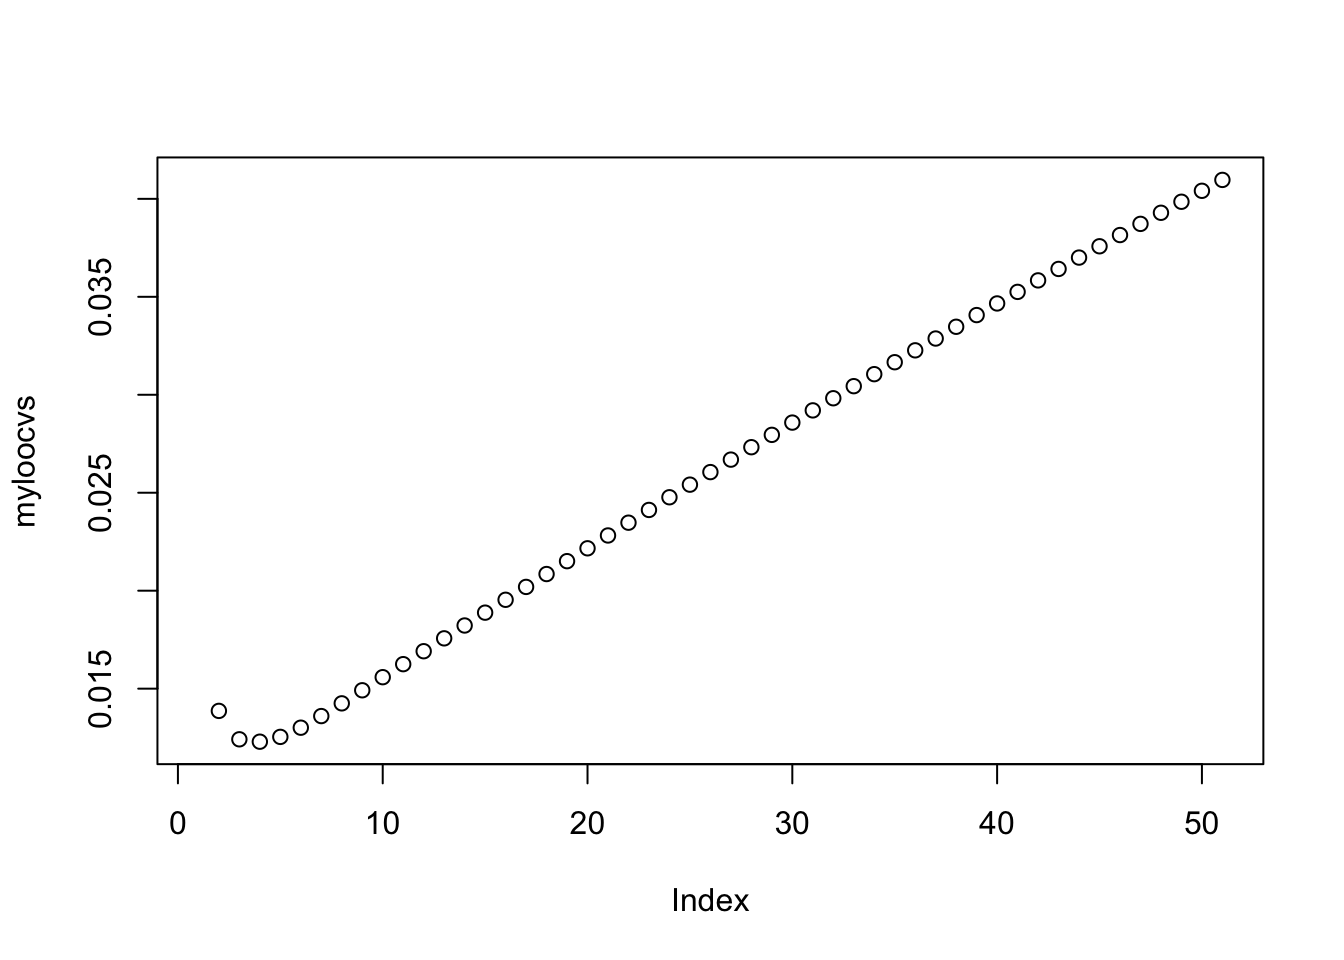
\includegraphics{hw1_files/figure-latex/unnamed-chunk-8-1.pdf}

\subsection{Select bandwidth using gcv function \& Fit with optimal
h}\label{select-bandwidth-using-gcv-function-fit-with-optimal-h}

\begin{Shaded}
\begin{Highlighting}[]
\NormalTok{## use GCV to choose bandwidth}
\NormalTok{alphamat =}\StringTok{ }\KeywordTok{matrix}\NormalTok{(}\DecValTok{0}\NormalTok{,}\DataTypeTok{ncol =} \DecValTok{2}\NormalTok{, }\DataTypeTok{nrow =} \DecValTok{100}\NormalTok{)}
\NormalTok{alphamat[,}\DecValTok{2}\NormalTok{] =}\StringTok{ }\KeywordTok{seq}\NormalTok{(}\DecValTok{0}\NormalTok{,}\DecValTok{1}\NormalTok{, }\DataTypeTok{length =} \DecValTok{100}\NormalTok{)}

\NormalTok{gcvs =}\StringTok{ }\KeywordTok{gcvplot}\NormalTok{(ys}\OperatorTok{~}\NormalTok{Xs,}\DataTypeTok{alpha =}\NormalTok{ alphamat)}
\KeywordTok{plot}\NormalTok{(gcvs}\OperatorTok{$}\NormalTok{alpha[,}\DecValTok{2}\NormalTok{], gcvs}\OperatorTok{$}\NormalTok{values)}
\end{Highlighting}
\end{Shaded}

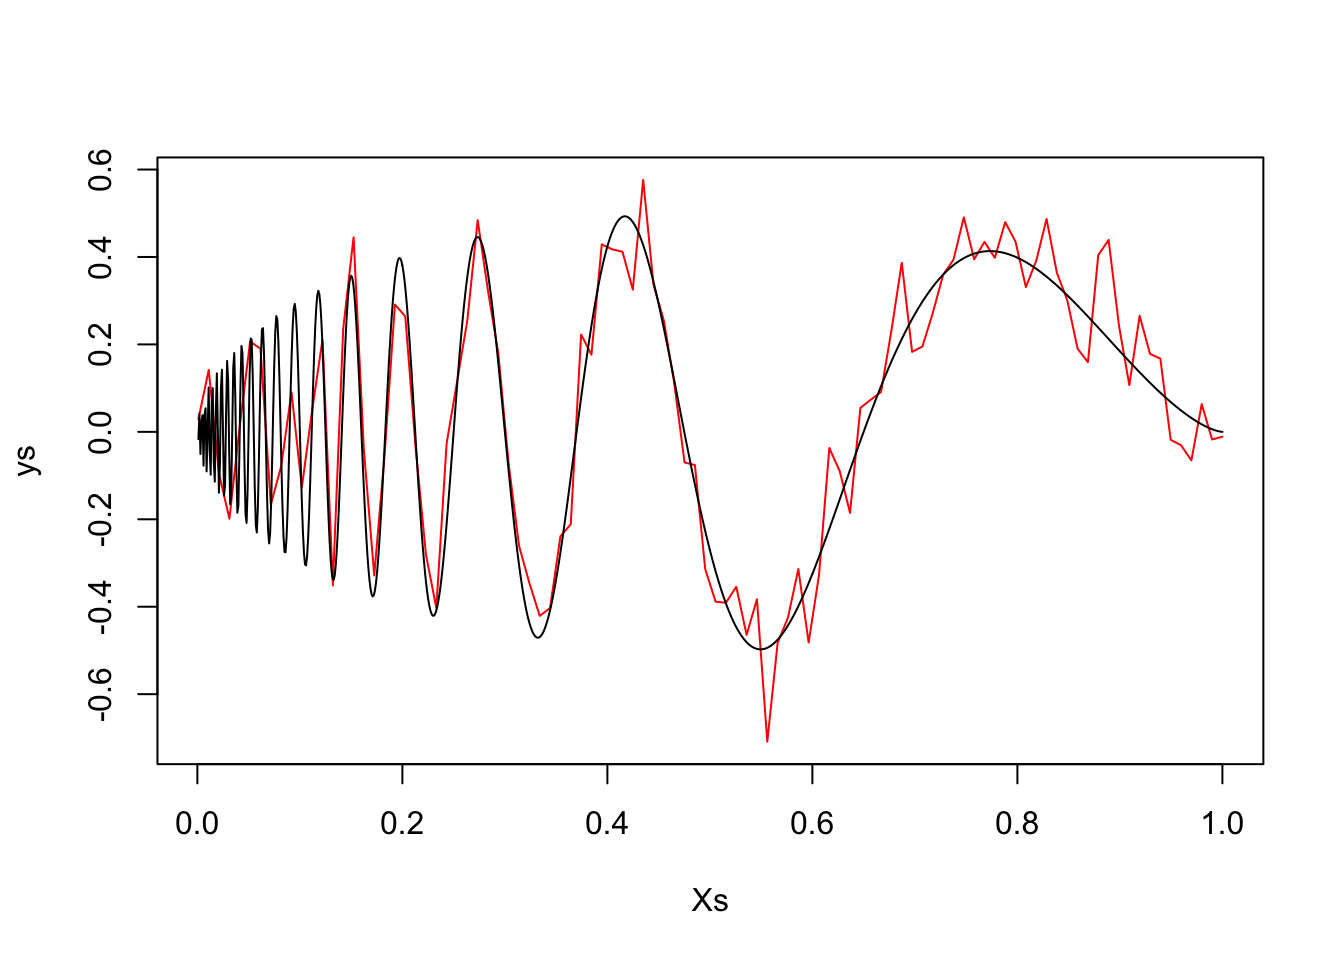
\includegraphics{hw1_files/figure-latex/unnamed-chunk-9-1.pdf}

\begin{Shaded}
\begin{Highlighting}[]
\NormalTok{optband2 =}\StringTok{ }\NormalTok{gcvs}\OperatorTok{$}\NormalTok{alpha[}\KeywordTok{which.min}\NormalTok{(gcvs}\OperatorTok{$}\NormalTok{values),}\DecValTok{2}\NormalTok{]}
\NormalTok{locfitopt2 =}\StringTok{ }\KeywordTok{locfit}\NormalTok{(ys}\OperatorTok{~}\NormalTok{Xs,}\DataTypeTok{alpha=} \KeywordTok{c}\NormalTok{(}\DecValTok{0}\NormalTok{,optband2))}

\KeywordTok{plot}\NormalTok{(Xs, ys)}
\KeywordTok{lines}\NormalTok{(Xs,}\KeywordTok{predict}\NormalTok{(locfitopt2, }\DataTypeTok{newdata =}\NormalTok{ Xs), }\DataTypeTok{type =} \StringTok{"l"}\NormalTok{,}\DataTypeTok{col =} \StringTok{"red"}\NormalTok{)}
\end{Highlighting}
\end{Shaded}

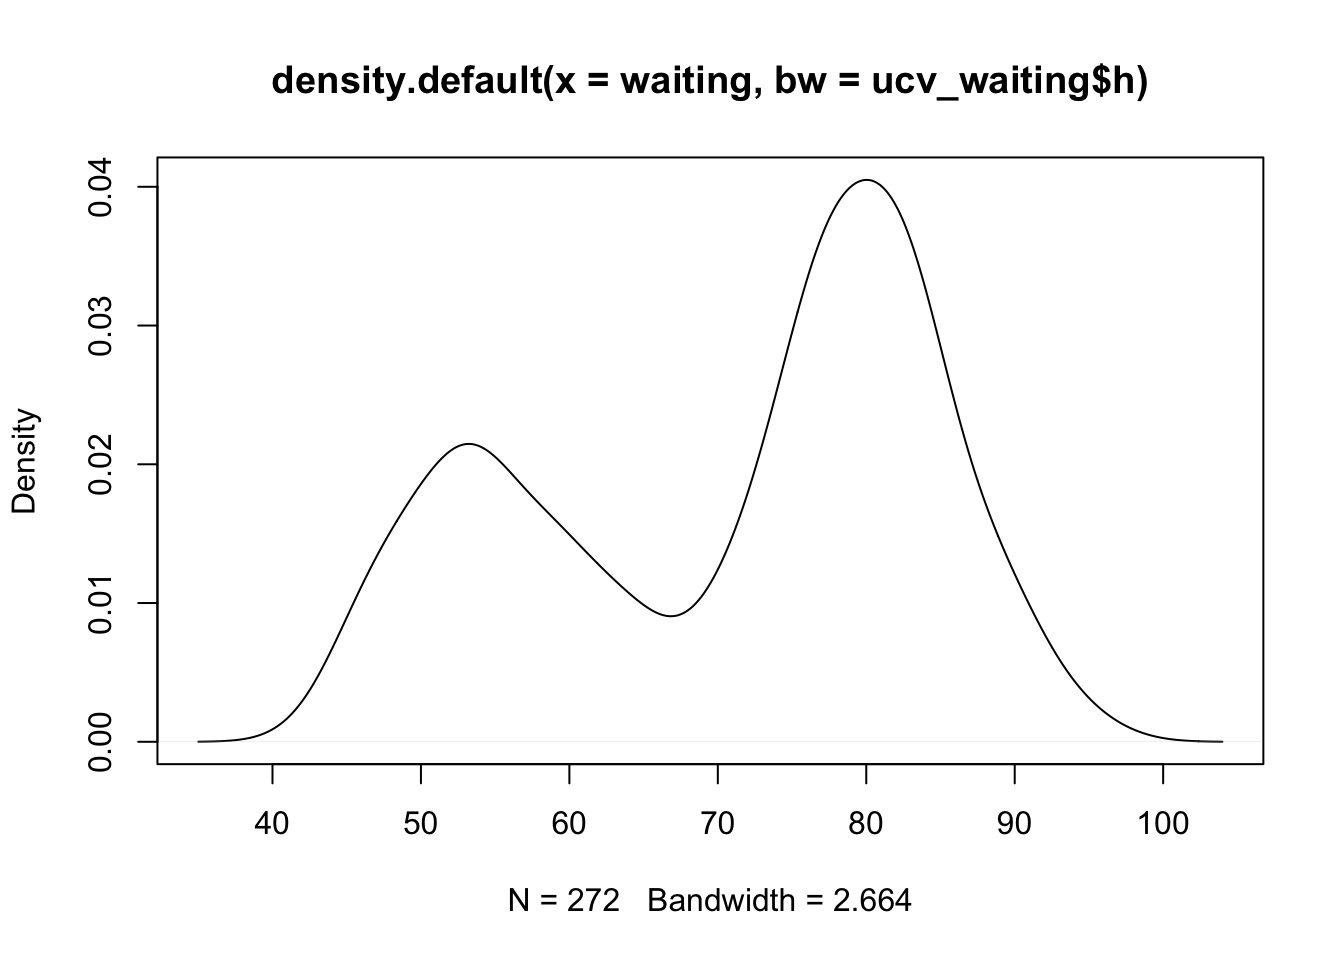
\includegraphics{hw1_files/figure-latex/unnamed-chunk-9-2.pdf}

\begin{Shaded}
\begin{Highlighting}[]
\NormalTok{nu =}\StringTok{ }\NormalTok{locfitopt2}\OperatorTok{$}\NormalTok{dp[[}\StringTok{"df1"}\NormalTok{]]}
\NormalTok{nutilde =}\StringTok{ }\NormalTok{locfitopt2}\OperatorTok{$}\NormalTok{dp[[}\StringTok{"df2"}\NormalTok{]]}
\NormalTok{sigmahat_sqrt =}\StringTok{ }\KeywordTok{sum}\NormalTok{(}\KeywordTok{residuals}\NormalTok{(locfitopt2)}\OperatorTok{^}\DecValTok{2}\NormalTok{)}\OperatorTok{/}\NormalTok{(N }\OperatorTok{-}\StringTok{ }\DecValTok{2}\OperatorTok{*}\NormalTok{nu }\OperatorTok{+}\StringTok{ }\NormalTok{nutilde)}

\NormalTok{diaghat =}\StringTok{ }\KeywordTok{predict}\NormalTok{(locfitopt2,}\DataTypeTok{where=}\StringTok{"data"}\NormalTok{,}\DataTypeTok{what=}\StringTok{"infl"}\NormalTok{) ## L_ii}
\NormalTok{normell =}\StringTok{ }\KeywordTok{predict}\NormalTok{(locfitopt2,}\DataTypeTok{where=}\StringTok{"data"}\NormalTok{,}\DataTypeTok{what=}\StringTok{"vari"}\NormalTok{) ## |l_i(x)|}

\NormalTok{critval =}\StringTok{ }\FloatTok{1.96}
\NormalTok{xg =}\StringTok{ }\NormalTok{Xs}
\NormalTok{pred =}\StringTok{ }\KeywordTok{predict}\NormalTok{(locfitopt2, }\DataTypeTok{newdata =}\NormalTok{ xg)}

\NormalTok{width =}\StringTok{ }\NormalTok{critval }\OperatorTok{*}\StringTok{ }\KeywordTok{sqrt}\NormalTok{(sigmahat_sqrt}\OperatorTok{*}\NormalTok{normell)}
\NormalTok{upper =}\StringTok{ }\NormalTok{pred }\OperatorTok{+}\StringTok{ }\NormalTok{width}
\NormalTok{lower =}\StringTok{ }\NormalTok{pred }\OperatorTok{-}\StringTok{ }\NormalTok{width}


\NormalTok{## plot confidence band}
\KeywordTok{plot}\NormalTok{(xg, pred,}\DataTypeTok{lwd=}\DecValTok{3}\NormalTok{, }\DataTypeTok{xlab=}\StringTok{"l"}\NormalTok{,}\DataTypeTok{ylab=}\StringTok{"Cl"}\NormalTok{,}\DataTypeTok{cex=}\DecValTok{3}\NormalTok{,}\DataTypeTok{cex.axis=}\FloatTok{1.3}\NormalTok{, }\DataTypeTok{cex.lab=}\FloatTok{1.3}\NormalTok{,}\DataTypeTok{type=}\StringTok{"l"}\NormalTok{)}
\KeywordTok{lines}\NormalTok{(xg, upper,}\DataTypeTok{col =} \DecValTok{2}\NormalTok{, }\DataTypeTok{lwd =} \DecValTok{3}\NormalTok{)}
\KeywordTok{lines}\NormalTok{(xg, lower,}\DataTypeTok{col =} \DecValTok{3}\NormalTok{, }\DataTypeTok{lwd =} \DecValTok{2}\NormalTok{)}
\end{Highlighting}
\end{Shaded}

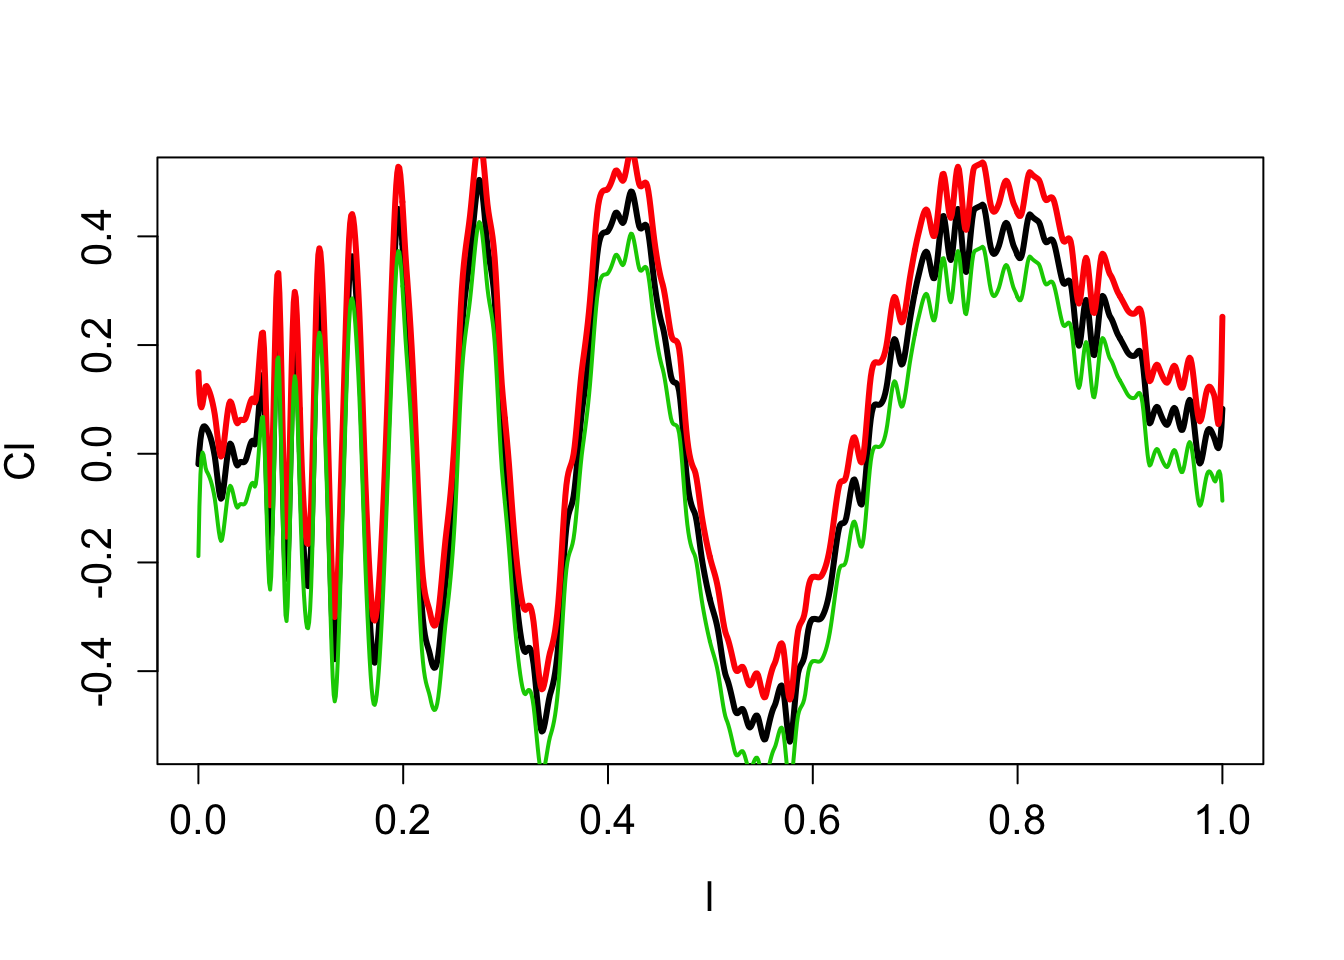
\includegraphics{hw1_files/figure-latex/unnamed-chunk-9-3.pdf}

\subsection{\texorpdfstring{Is In(x) the 95\% CI for
\(r(x)\)}{Is In(x) the 95\% CI for r(x)}}\label{is-inx-the-95-ci-for-rx}

No. In(x) is centered around \(E(\hat{r}(x))\), which is not \(r(x)\).
This CI is computed by the fact that for a fixed x, \(\hat{r}(x)\)
asympototically follows \(N(E(\hat{r}(x)), \hat{\sigma}(x))\). That
correctness of the claim requires \(E(\hat{r}(x)) = r(x)\), which is
apparently violated.

\section{3. Kernel density estimate for Old Faithful
Geyser}\label{kernel-density-estimate-for-old-faithful-geyser}

\begin{Shaded}
\begin{Highlighting}[]
\KeywordTok{data}\NormalTok{(}\StringTok{"faithful"}\NormalTok{)}
\KeywordTok{attach}\NormalTok{(faithful)}

\KeywordTok{library}\NormalTok{(kedd)}
\NormalTok{## Broad search}
\NormalTok{ucv_eruptions =}\StringTok{ }\KeywordTok{h.ucv}\NormalTok{(eruptions)}
\KeywordTok{plot}\NormalTok{(ucv_eruptions)}
\end{Highlighting}
\end{Shaded}

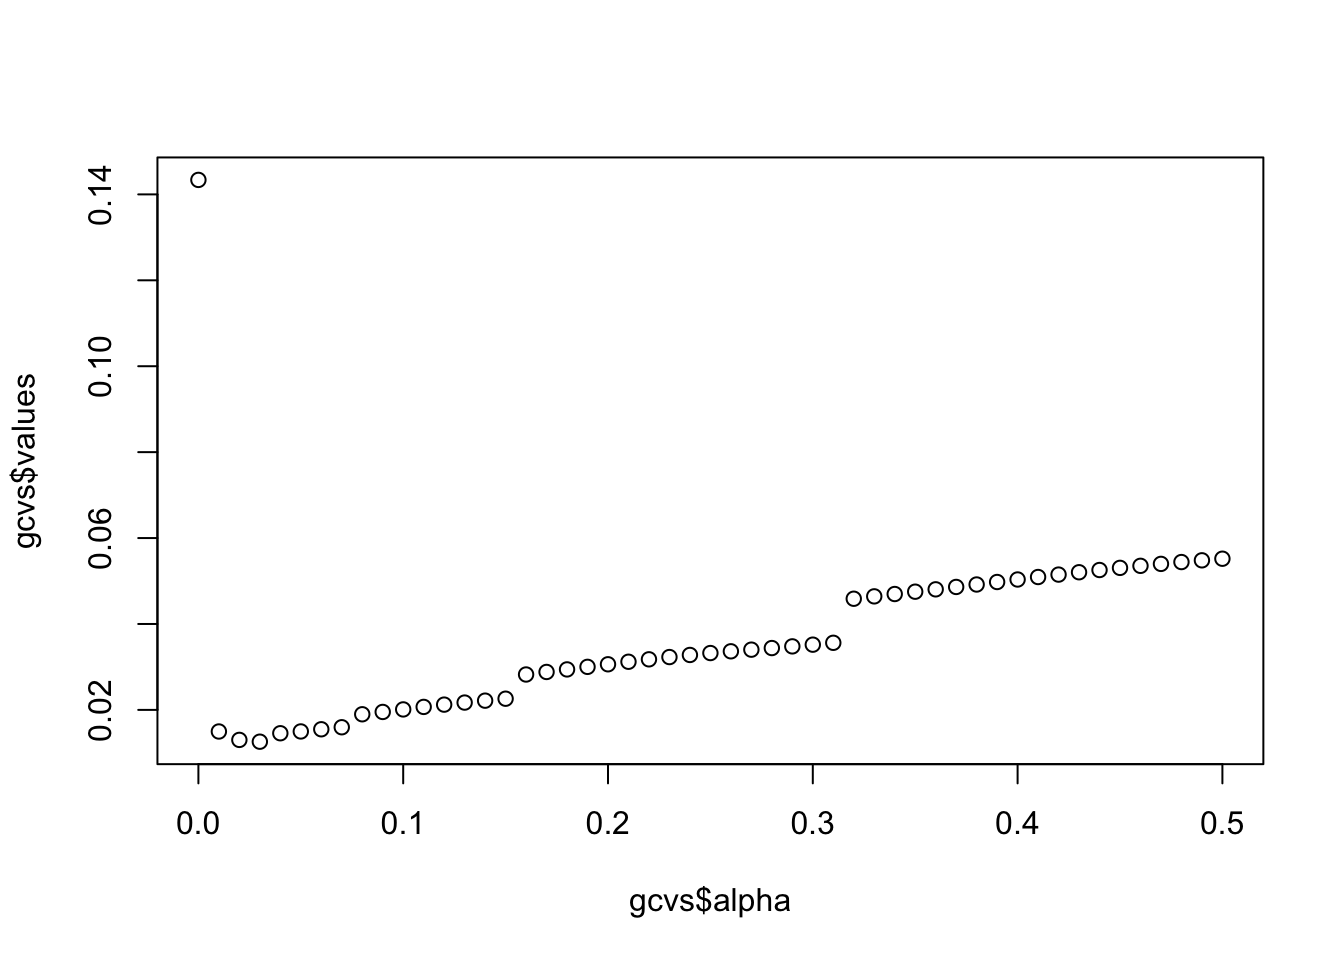
\includegraphics{hw1_files/figure-latex/unnamed-chunk-10-1.pdf}

\begin{verbatim}
## $kernel
## [1] "gaussian"
## 
## $deriv.order
## [1] 0
## 
## $seq.bws
##  [1] 0.06382504 0.07988984 0.09595465 0.11201945 0.12808426 0.14414906
##  [7] 0.16021387 0.17627867 0.19234348 0.20840828 0.22447309 0.24053789
## [13] 0.25660269 0.27266750 0.28873230 0.30479711 0.32086191 0.33692672
## [19] 0.35299152 0.36905633 0.38512113 0.40118594 0.41725074 0.43331555
## [25] 0.44938035 0.46544516 0.48150996 0.49757477 0.51363957 0.52970438
## [31] 0.54576918 0.56183399 0.57789879 0.59396360 0.61002840 0.62609321
## [37] 0.64215801 0.65822282 0.67428762 0.69035243 0.70641723 0.72248204
## [43] 0.73854684 0.75461165 0.77067645 0.78674126 0.80280606 0.81887087
## [49] 0.83493567 0.85100048
## 
## $ucv
##  [1] -0.4232268 -0.4258325 -0.4268588 -0.4268189 -0.4259983 -0.4246085
##  [7] -0.4228091 -0.4207043 -0.4183518 -0.4157788 -0.4129965 -0.4100111
## [13] -0.4068286 -0.4034573 -0.3999082 -0.3961946 -0.3923311 -0.3883332
## [19] -0.3842161 -0.3799950 -0.3756846 -0.3712988 -0.3668511 -0.3623543
## [25] -0.3578208 -0.3532625 -0.3486911 -0.3441178 -0.3395537 -0.3350094
## [31] -0.3304954 -0.3260215 -0.3215974 -0.3172321 -0.3129343 -0.3087120
## [37] -0.3045724 -0.3005222 -0.2965672 -0.2927126 -0.2889626 -0.2853210
## [43] -0.2817903 -0.2783726 -0.2750693 -0.2718809 -0.2688074 -0.2658482
## [49] -0.2630020 -0.2602672
\end{verbatim}

\begin{Shaded}
\begin{Highlighting}[]
\NormalTok{## fine search (locate a neighborhood of the best point from broad search)}
\NormalTok{ucv_eruptions =}\StringTok{ }\KeywordTok{h.ucv}\NormalTok{(eruptions, }\DataTypeTok{lower =} \FloatTok{0.7}\OperatorTok{*}\NormalTok{ucv_eruptions}\OperatorTok{$}\NormalTok{h, }\DataTypeTok{higher =} \FloatTok{1.3}\OperatorTok{*}\NormalTok{ucv_eruptions}\OperatorTok{$}\NormalTok{h, }\DataTypeTok{tol =} \FloatTok{0.0001}\NormalTok{)}

\NormalTok{## Broad search}
\NormalTok{ucv_waiting =}\StringTok{ }\KeywordTok{h.ucv}\NormalTok{(waiting)}
\KeywordTok{plot}\NormalTok{(ucv_waiting)}
\end{Highlighting}
\end{Shaded}

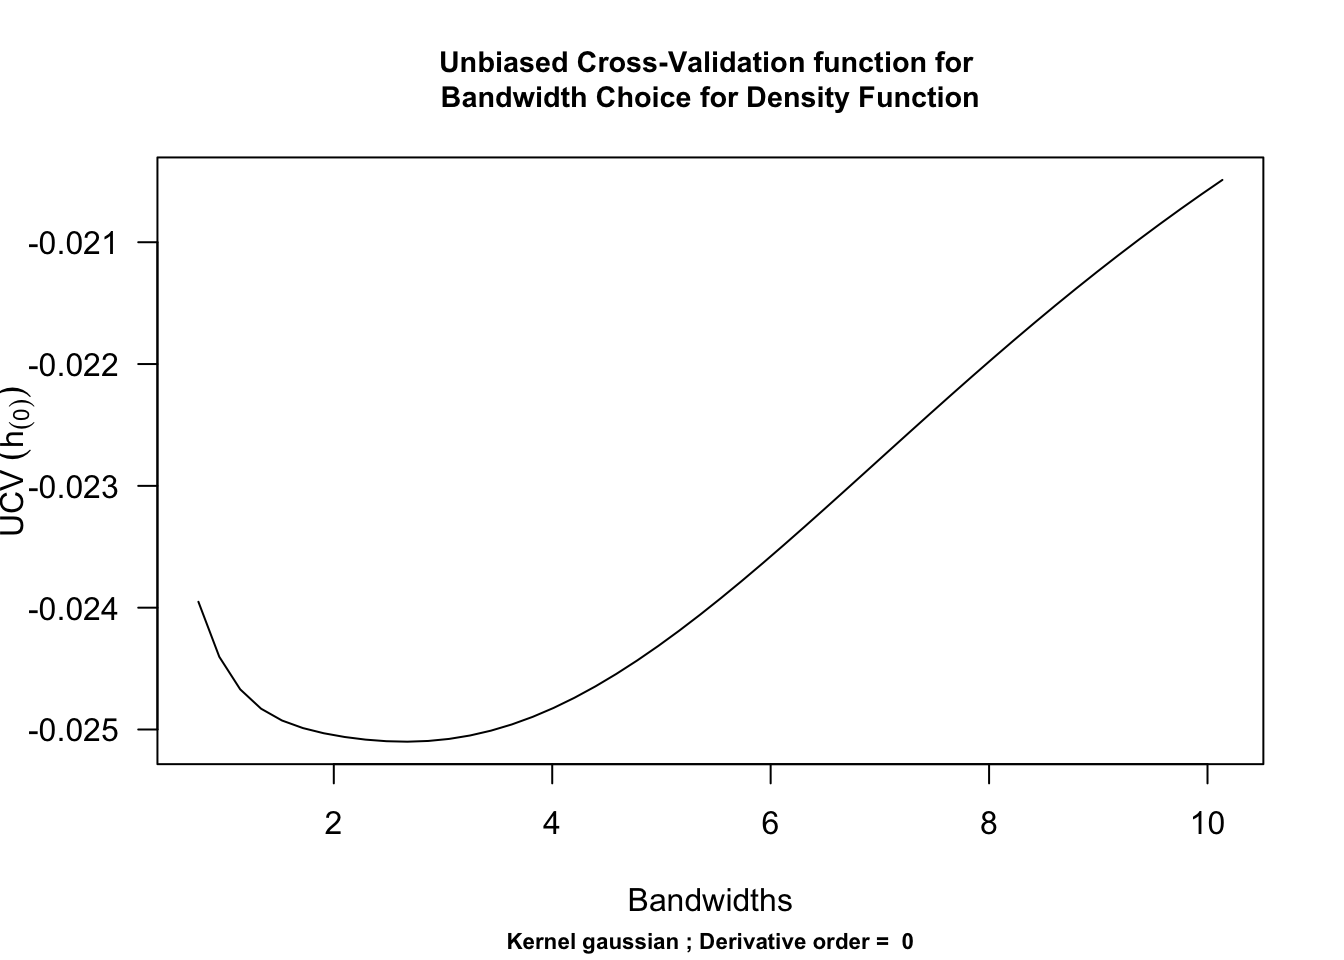
\includegraphics{hw1_files/figure-latex/unnamed-chunk-10-2.pdf}

\begin{verbatim}
## $kernel
## [1] "gaussian"
## 
## $deriv.order
## [1] 0
## 
## $seq.bws
##  [1]  0.7602256  0.9515749  1.1429243  1.3342736  1.5256229  1.7169722
##  [7]  1.9083215  2.0996708  2.2910201  2.4823694  2.6737187  2.8650681
## [13]  3.0564174  3.2477667  3.4391160  3.6304653  3.8218146  4.0131639
## [19]  4.2045132  4.3958625  4.5872118  4.7785612  4.9699105  5.1612598
## [25]  5.3526091  5.5439584  5.7353077  5.9266570  6.1180063  6.3093556
## [31]  6.5007050  6.6920543  6.8834036  7.0747529  7.2661022  7.4574515
## [37]  7.6488008  7.8401501  8.0314994  8.2228487  8.4141981  8.6055474
## [43]  8.7968967  8.9882460  9.1795953  9.3709446  9.5622939  9.7536432
## [49]  9.9449925 10.1363419
## 
## $ucv
##  [1] -0.02395152 -0.02440334 -0.02467032 -0.02482935 -0.02492616
##  [6] -0.02498823 -0.02503085 -0.02506151 -0.02508310 -0.02509613
## [11] -0.02510007 -0.02509402 -0.02507721 -0.02504910 -0.02500946
## [16] -0.02495830 -0.02489589 -0.02482263 -0.02473907 -0.02464581
## [21] -0.02454353 -0.02443293 -0.02431474 -0.02418970 -0.02405855
## [26] -0.02392202 -0.02378083 -0.02363570 -0.02348733 -0.02333637
## [31] -0.02318346 -0.02302922 -0.02287421 -0.02271897 -0.02256400
## [36] -0.02240976 -0.02225667 -0.02210509 -0.02195537 -0.02180779
## [41] -0.02166261 -0.02152005 -0.02138029 -0.02124346 -0.02110968
## [46] -0.02097903 -0.02085156 -0.02072730 -0.02060626 -0.02048841
\end{verbatim}

\begin{Shaded}
\begin{Highlighting}[]
\NormalTok{## fine search (locate a neighborhood of the best point from broad search)}
\NormalTok{ucv_waiting =}\StringTok{ }\KeywordTok{h.ucv}\NormalTok{(waiting, }\DataTypeTok{lower =} \FloatTok{0.8}\OperatorTok{*}\NormalTok{ucv_waiting}\OperatorTok{$}\NormalTok{h, }\DataTypeTok{higher =} \FloatTok{1.2}\OperatorTok{*}\NormalTok{ucv_waiting}\OperatorTok{$}\NormalTok{h,}\DataTypeTok{tol =} \FloatTok{0.0001}\NormalTok{)}
\end{Highlighting}
\end{Shaded}

\subsection{plot estimated density with optimum
h}\label{plot-estimated-density-with-optimum-h}

\begin{Shaded}
\begin{Highlighting}[]
\KeywordTok{plot}\NormalTok{(}\KeywordTok{density}\NormalTok{(eruptions, }\DataTypeTok{bw =}\NormalTok{ ucv_eruptions}\OperatorTok{$}\NormalTok{h))}
\end{Highlighting}
\end{Shaded}

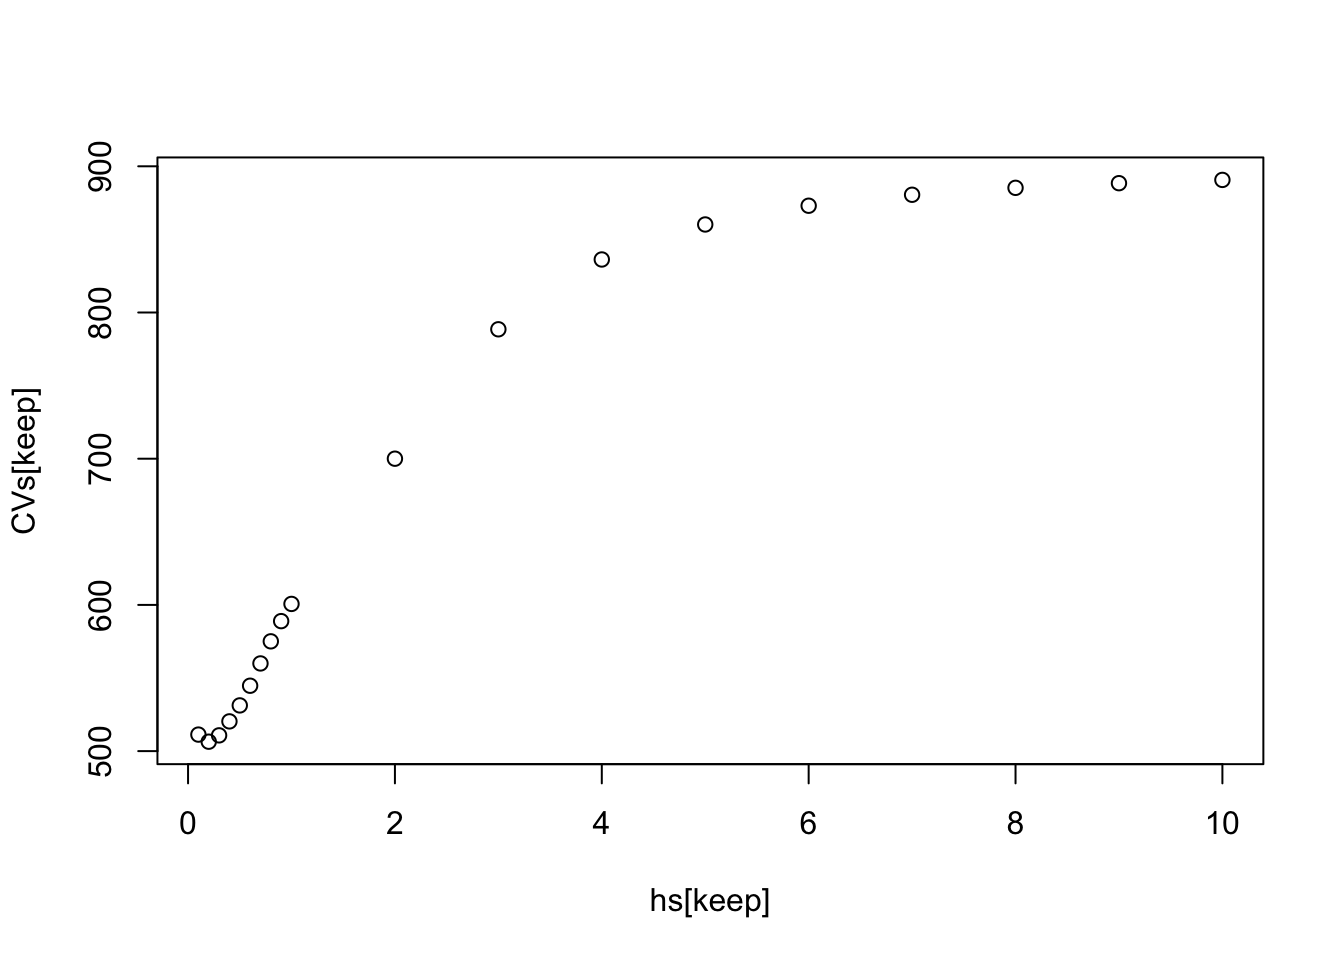
\includegraphics{hw1_files/figure-latex/unnamed-chunk-11-1.pdf}

\begin{Shaded}
\begin{Highlighting}[]
\KeywordTok{plot}\NormalTok{(}\KeywordTok{density}\NormalTok{(waiting, }\DataTypeTok{bw =}\NormalTok{ ucv_waiting}\OperatorTok{$}\NormalTok{h))}
\end{Highlighting}
\end{Shaded}

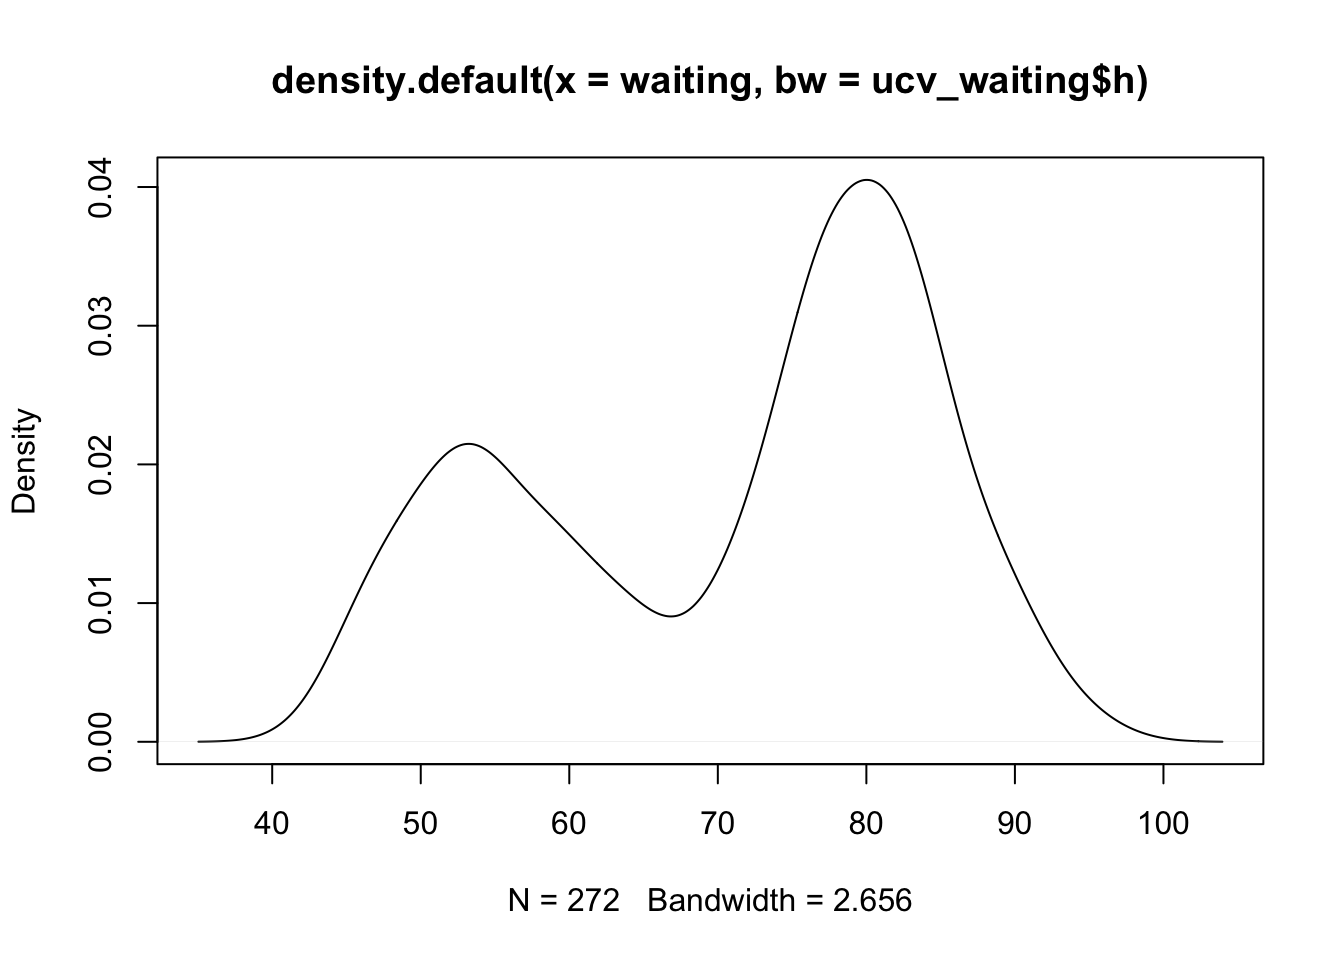
\includegraphics{hw1_files/figure-latex/unnamed-chunk-11-2.pdf}

\section{4 Risk of a two-dimensional Kernel density
estimate}\label{risk-of-a-two-dimensional-kernel-density-estimate}

Let
\(K_h(x,y,X,Y) := \frac{1}{h^2} E(K(\frac{X-x}{h})K(\frac{Y-y}{h}))\)

By \(|\Pr(x,y) - p(x-uh,y-vh) < L(|uh|^\beta + |vh|^\beta|)\), we have
\(\Pr(x-uh,y-uh) < \Pr(x,y) + Lh^\beta(|u|^\beta+|v|^\beta)\)

Thus: \[
E(\hat{\Pr(x,y)}) = \frac{1}{h^2} E(K_h(x,y,X,Y)) \\
= \frac{1}{h^2} \int K(\frac{X-x}{h}) K(\frac{Y-y}{h}) \Pr(X,Y)dXdY \\
= \int K(u) K(v) P(x-Uh, y-Vh)dUdV \\
(U := \frac{x-X}{h})\\
\le \int K(u) K(v) (P(x,y) + Lh^\beta(|u|^\beta+|v|^\beta))dUdV \\
= \Pr(x,y) + Lh^\beta \int K(u)K(v)(|u|^\beta+|v|^\beta)dUdV\\
= \Pr(x,y) + Lh^\beta M \\
(M := \int K(u)K(v)(|u|^\beta+|v|^\beta)dUdV)
\] Thus we have
\(bias(x,y) = E(\hat{P_n}(x,y)) - \Pr(x,y) <= MLh^\beta\)

Similarly, for variance, \[
Var(\hat{P_n}(x,y)) = \frac{1}{n} Var(K_h(x,y,X,Y))\\
\leq \frac{1}{n} E(K_h(x,y,X,Y)^2)\\
= \frac{1}{nh^4} \int K^2(\frac{X-x}{h}) K^2(\frac{Y-y}{h}) \Pr(X,Y)dXdY \\
= \frac{1}{nh^2} \int K^2(U) K^2(V) \Pr(x-Uh,y-Vh)dUdV \\
\leq \frac{1}{nh^2} (\int K^2(U) K^2(V)dUdV + Lh^\beta \int K^2(U)K^2(V) (|U|^\beta + |V|^\beta))dUdV)\\
\leq \frac{M_2}{nh^2} \Pr(x,y)\\
(M_2 := \frac{1}{nh^2} (\int K^2(U) K^2(V)dUdV)
\]

Thus we have \(V(x,y) \leq \frac{M_2\Pr(x,y)}{nh^2}\)\\
It is also easy to check both \(M\) and \(M_2\) are not inifinity.\\
\[
Risk(x,y) = bias(x,y)^2 + V(x,y) \leq (MLh^\beta)^2 + \frac{M_2\Pr(x,y)}{nh^2} := H(h) \\
h^* = (\frac{M_2\Pr(x,y)}{ML^2}) = O((\frac{1}{n})^\frac{1}{2\beta+2})\\
H(h^*) = O(\frac{1}{n})^\frac{\beta}{\beta+1}
\] Thus set \(H(h^*) < \epsilon\), we have the rate of convergence as
\(O(\epsilon ^ -\frac{\beta+1}{\beta})\)

\section{5 Capital Bike Sharing}\label{capital-bike-sharing}

\begin{Shaded}
\begin{Highlighting}[]
\NormalTok{data =}\StringTok{ }\KeywordTok{read.csv}\NormalTok{(}\StringTok{"../data/hw1/train.csv"}\NormalTok{)}
\NormalTok{test =}\StringTok{ }\KeywordTok{read.csv}\NormalTok{(}\StringTok{"../data/hw1/test.csv"}\NormalTok{)}

\CommentTok{#fac_names = c("holiday","workingday","weather")}
\CommentTok{# fac_names = c("holiday","workingday","weather","season","year","hour")}
\NormalTok{fac_names =}\StringTok{ }\KeywordTok{c}\NormalTok{(}\StringTok{"holiday"}\NormalTok{,}\StringTok{"workingday"}\NormalTok{,}\StringTok{"weather"}\NormalTok{,}\StringTok{"season"}\NormalTok{,}\StringTok{"year"}\NormalTok{,}\StringTok{"hour"}\NormalTok{)}

\ControlFlowTok{for}\NormalTok{(i }\ControlFlowTok{in} \DecValTok{1}\OperatorTok{:}\KeywordTok{length}\NormalTok{(fac_names))\{}
\NormalTok{  name =}\StringTok{ }\NormalTok{fac_names[i]}
\NormalTok{  data[[name]] =}\StringTok{ }\KeywordTok{factor}\NormalTok{(data[[name]])}
\NormalTok{  test[[name]] =}\StringTok{ }\KeywordTok{factor}\NormalTok{(test[[name]])}
\NormalTok{\}}
\NormalTok{data[[}\StringTok{"transformed_count"}\NormalTok{]] =}\StringTok{ }\KeywordTok{log}\NormalTok{(data}\OperatorTok{$}\NormalTok{count }\OperatorTok{+}\StringTok{ }\DecValTok{1}\NormalTok{)}

\NormalTok{## split train into train and validation}
\NormalTok{train =}\StringTok{ }\NormalTok{data[data}\OperatorTok{$}\NormalTok{day }\OperatorTok{<}\StringTok{ }\DecValTok{16}\NormalTok{,]}
\NormalTok{val =}\StringTok{ }\NormalTok{data[data}\OperatorTok{$}\NormalTok{day }\OperatorTok{>}\StringTok{ }\DecValTok{15}\NormalTok{,]}

\NormalTok{## define loss}
\NormalTok{RMSLE_log <-}\StringTok{ }\ControlFlowTok{function}\NormalTok{(count_log,count_hat_log)\{}
  \KeywordTok{return}\NormalTok{(}\KeywordTok{sqrt}\NormalTok{(}\KeywordTok{mean}\NormalTok{((count_log}\OperatorTok{-}\NormalTok{count_hat_log)}\OperatorTok{^}\DecValTok{2}\NormalTok{)))}
\NormalTok{\}}
\end{Highlighting}
\end{Shaded}

\begin{Shaded}
\begin{Highlighting}[]
\CommentTok{#plot(density(train$count))}
\KeywordTok{hist}\NormalTok{(train}\OperatorTok{$}\NormalTok{count)}
\end{Highlighting}
\end{Shaded}

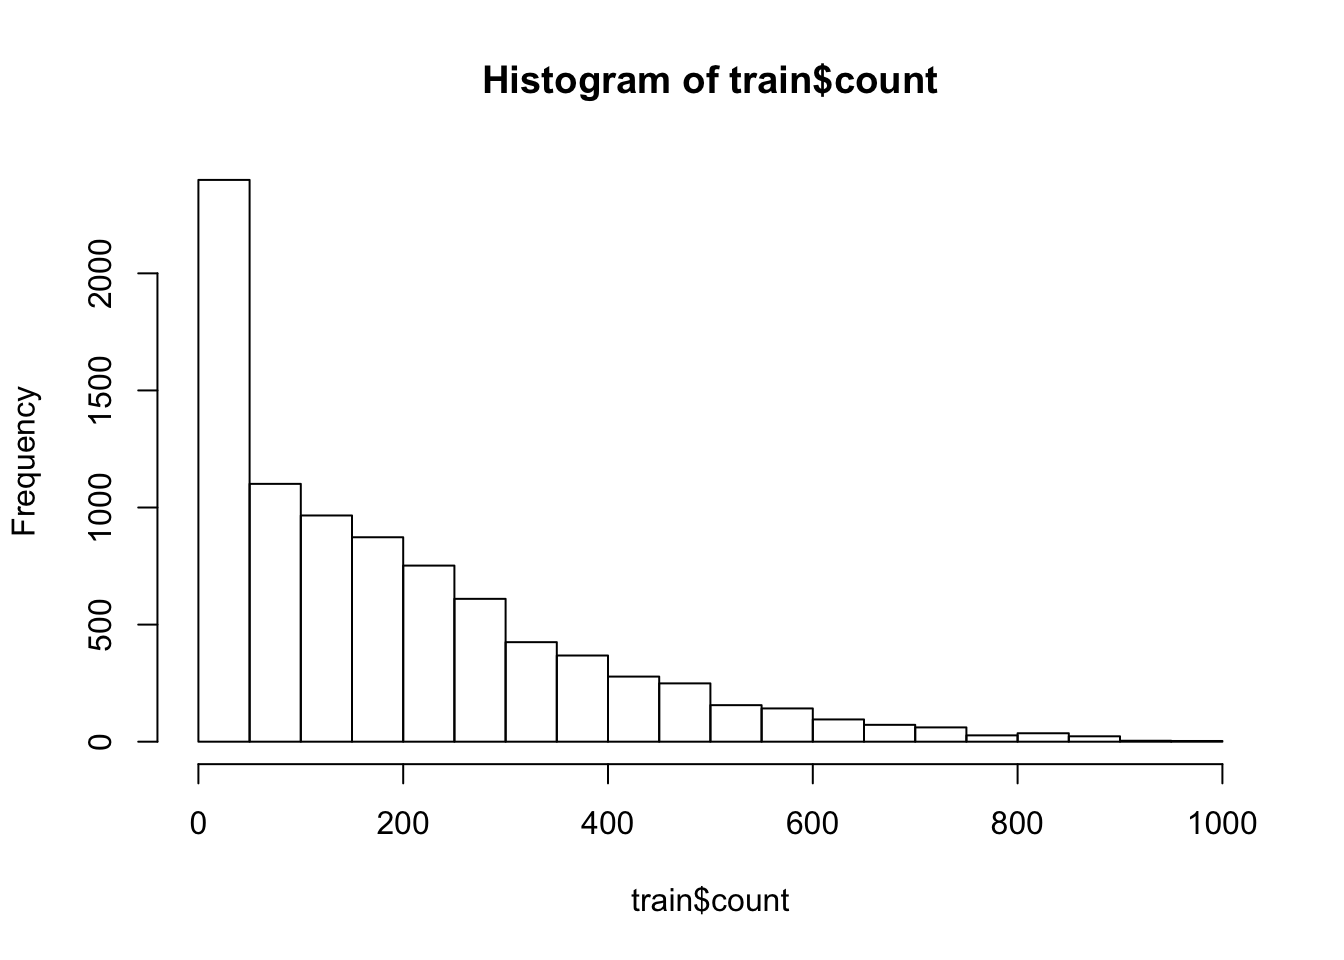
\includegraphics{hw1_files/figure-latex/unnamed-chunk-13-1.pdf}

\begin{Shaded}
\begin{Highlighting}[]
\CommentTok{# p1 = ggplot(train,aes(atemp, count, color = weather)) + }
\CommentTok{#   geom_point()}
\CommentTok{# }
\CommentTok{# p2 = ggplot(train,aes(humidity,count,  color = weather)) + }
\CommentTok{#   geom_point()}
\CommentTok{# }
\CommentTok{# p3 = ggplot(train,aes(windspeed,count,  color = weather)) + }
\CommentTok{#   geom_point()}

\NormalTok{p1 <-}\StringTok{ }\KeywordTok{ggplot}\NormalTok{(}\KeywordTok{subset}\NormalTok{(train,workingday}\OperatorTok{==}\DecValTok{1}\NormalTok{),}\KeywordTok{aes}\NormalTok{(hour,count)) }\OperatorTok{+}\StringTok{ }
\StringTok{  }\KeywordTok{geom_point}\NormalTok{()}

\NormalTok{p2 <-}\StringTok{ }\KeywordTok{ggplot}\NormalTok{(}\KeywordTok{subset}\NormalTok{(train,workingday}\OperatorTok{==}\DecValTok{0}\NormalTok{),}\KeywordTok{aes}\NormalTok{(hour,count)) }\OperatorTok{+}\StringTok{ }
\StringTok{  }\KeywordTok{geom_point}\NormalTok{()}

\KeywordTok{grid.arrange}\NormalTok{(p1,p2,}\DataTypeTok{nrow =} \DecValTok{2}\NormalTok{)}
\end{Highlighting}
\end{Shaded}

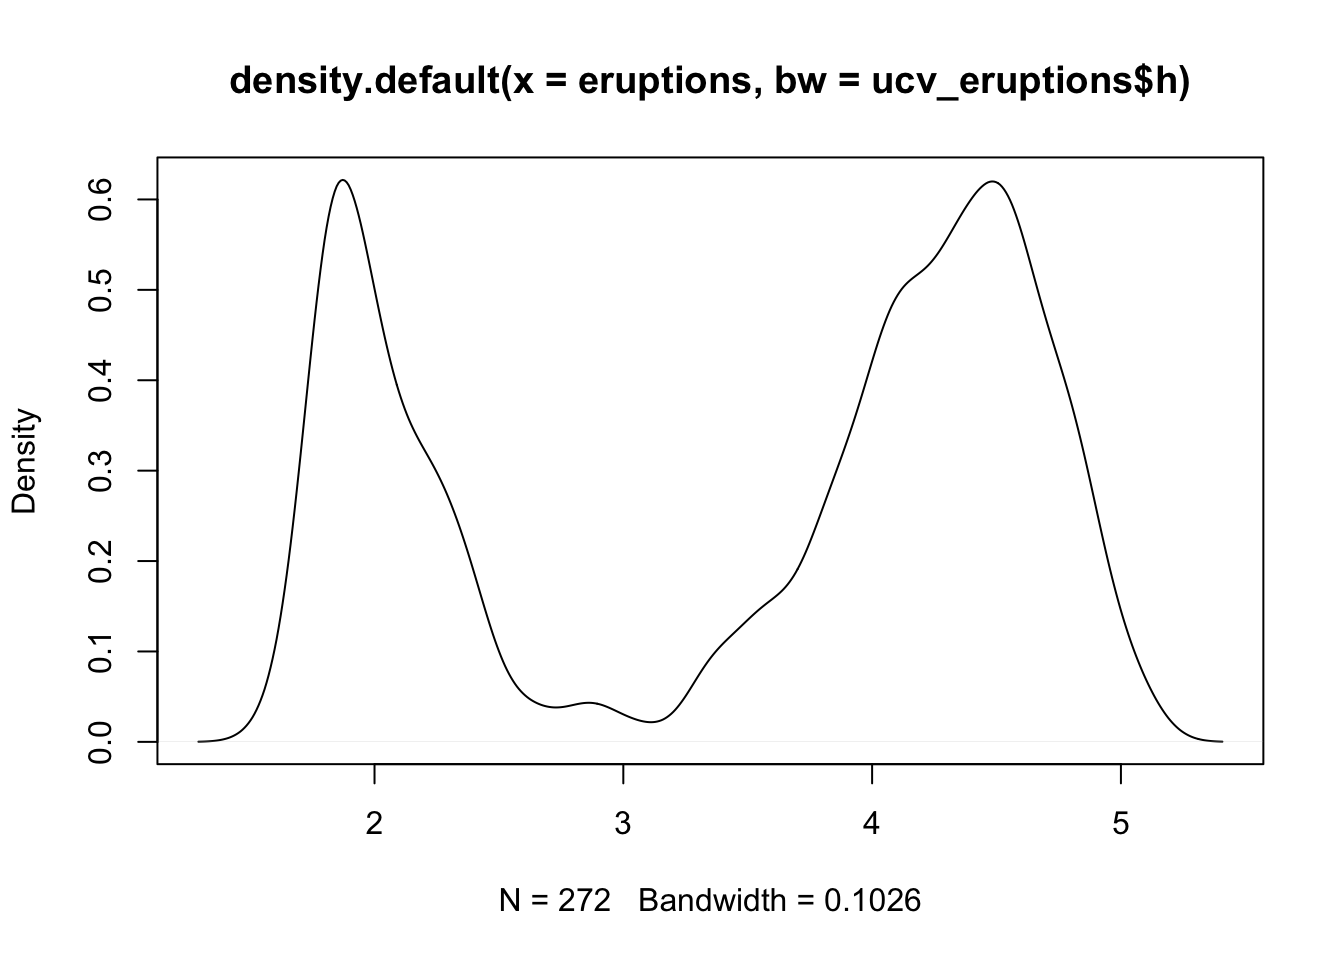
\includegraphics{hw1_files/figure-latex/unnamed-chunk-14-1.pdf} \#\#\#
Comment: The counts distribution with hours are different for workingday
and nonworkingday. So there is a very strong connection between the
interaction between hour and workingday! Other factors do not bring
about too much difference

\subsection{(a) linear model on count}\label{a-linear-model-on-count}

\begin{Shaded}
\begin{Highlighting}[]
\NormalTok{linearMD <-}\KeywordTok{lm}\NormalTok{(transformed_count}\OperatorTok{~}\NormalTok{daylabel}\OperatorTok{+}\NormalTok{workingday}\OperatorTok{*}\NormalTok{hour }\OperatorTok{+}\StringTok{ }\NormalTok{season }\OperatorTok{+}\NormalTok{atemp}\OperatorTok{+}\NormalTok{humidity}\OperatorTok{+}\NormalTok{windspeed,}\DataTypeTok{data=}\NormalTok{train)}
\KeywordTok{summary}\NormalTok{(linearMD)}
\end{Highlighting}
\end{Shaded}

\begin{verbatim}
## 
## Call:
## lm(formula = transformed_count ~ daylabel + workingday * hour + 
##     season + atemp + humidity + windspeed, data = train)
## 
## Residuals:
##     Min      1Q  Median      3Q     Max 
## -3.5205 -0.1618  0.0392  0.2168  2.3149 
## 
## Coefficients:
##                      Estimate Std. Error t value Pr(>|t|)    
## (Intercept)         3.564e+00  4.405e-02  80.918  < 2e-16 ***
## daylabel            1.329e-03  2.321e-05  57.267  < 2e-16 ***
## workingday1        -1.012e+00  4.447e-02 -22.763  < 2e-16 ***
## hour1              -2.378e-01  5.199e-02  -4.573 4.87e-06 ***
## hour2              -5.801e-01  5.199e-02 -11.157  < 2e-16 ***
## hour3              -1.269e+00  5.200e-02 -24.409  < 2e-16 ***
## hour4              -2.232e+00  5.202e-02 -42.911  < 2e-16 ***
## hour5              -2.253e+00  5.203e-02 -43.299  < 2e-16 ***
## hour6              -1.632e+00  5.204e-02 -31.362  < 2e-16 ***
## hour7              -7.776e-01  5.202e-02 -14.949  < 2e-16 ***
## hour8               8.747e-02  5.199e-02   1.682 0.092516 .  
## hour9               5.699e-01  5.200e-02  10.961  < 2e-16 ***
## hour10              9.405e-01  5.205e-02  18.068  < 2e-16 ***
## hour11              1.111e+00  5.214e-02  21.312  < 2e-16 ***
## hour12              1.240e+00  5.226e-02  23.723  < 2e-16 ***
## hour13              1.224e+00  5.237e-02  23.373  < 2e-16 ***
## hour14              1.181e+00  5.245e-02  22.519  < 2e-16 ***
## hour15              1.162e+00  5.244e-02  22.162  < 2e-16 ***
## hour16              1.150e+00  5.241e-02  21.936  < 2e-16 ***
## hour17              1.063e+00  5.232e-02  20.320  < 2e-16 ***
## hour18              9.181e-01  5.223e-02  17.578  < 2e-16 ***
## hour19              7.567e-01  5.212e-02  14.520  < 2e-16 ***
## hour20              5.231e-01  5.206e-02  10.049  < 2e-16 ***
## hour21              3.575e-01  5.202e-02   6.872 6.79e-12 ***
## hour22              1.770e-01  5.201e-02   3.403 0.000669 ***
## hour23             -1.187e-01  5.199e-02  -2.283 0.022460 *  
## season2             3.250e-01  1.599e-02  20.322  < 2e-16 ***
## season3             1.757e-01  2.060e-02   8.529  < 2e-16 ***
## season4             2.633e-01  1.458e-02  18.054  < 2e-16 ***
## atemp               2.943e-02  8.909e-04  33.030  < 2e-16 ***
## humidity           -6.140e-03  2.610e-04 -23.525  < 2e-16 ***
## windspeed          -5.585e-03  5.538e-04 -10.084  < 2e-16 ***
## workingday1:hour1  -5.475e-01  6.289e-02  -8.707  < 2e-16 ***
## workingday1:hour2  -8.184e-01  6.289e-02 -13.013  < 2e-16 ***
## workingday1:hour3  -5.404e-01  6.289e-02  -8.592  < 2e-16 ***
## workingday1:hour4   5.249e-01  6.289e-02   8.346  < 2e-16 ***
## workingday1:hour5   1.990e+00  6.289e-02  31.644  < 2e-16 ***
## workingday1:hour6   2.818e+00  6.289e-02  44.811  < 2e-16 ***
## workingday1:hour7   2.976e+00  6.289e-02  47.319  < 2e-16 ***
## workingday1:hour8   2.624e+00  6.289e-02  41.721  < 2e-16 ***
## workingday1:hour9   1.425e+00  6.289e-02  22.657  < 2e-16 ***
## workingday1:hour10  3.780e-01  6.289e-02   6.010 1.93e-09 ***
## workingday1:hour11  2.856e-01  6.289e-02   4.541 5.67e-06 ***
## workingday1:hour12  3.707e-01  6.289e-02   5.894 3.91e-09 ***
## workingday1:hour13  3.324e-01  6.290e-02   5.286 1.28e-07 ***
## workingday1:hour14  2.560e-01  6.289e-02   4.071 4.72e-05 ***
## workingday1:hour15  3.521e-01  6.290e-02   5.597 2.24e-08 ***
## workingday1:hour16  7.617e-01  6.289e-02  12.111  < 2e-16 ***
## workingday1:hour17  1.494e+00  6.289e-02  23.759  < 2e-16 ***
## workingday1:hour18  1.589e+00  6.289e-02  25.274  < 2e-16 ***
## workingday1:hour19  1.427e+00  6.289e-02  22.685  < 2e-16 ***
## workingday1:hour20  1.342e+00  6.289e-02  21.331  < 2e-16 ***
## workingday1:hour21  1.240e+00  6.290e-02  19.715  < 2e-16 ***
## workingday1:hour22  1.154e+00  6.290e-02  18.350  < 2e-16 ***
## workingday1:hour23  1.018e+00  6.289e-02  16.183  < 2e-16 ***
## ---
## Signif. codes:  0 '***' 0.001 '**' 0.01 '*' 0.05 '.' 0.1 ' ' 1
## 
## Residual standard error: 0.3925 on 8585 degrees of freedom
## Multiple R-squared:  0.9277, Adjusted R-squared:  0.9273 
## F-statistic:  2041 on 54 and 8585 DF,  p-value: < 2.2e-16
\end{verbatim}

\begin{Shaded}
\begin{Highlighting}[]
\CommentTok{#plot(linearMD)}
\end{Highlighting}
\end{Shaded}

\begin{Shaded}
\begin{Highlighting}[]
\CommentTok{# linearPredict = predict(linearMD, subset(val, colnames = c("atemp","humidity","windspeed","weather")))}
\NormalTok{linearPredict_train =}\StringTok{ }\KeywordTok{predict}\NormalTok{(linearMD, train)}
\NormalTok{linearPredict_val =}\StringTok{ }\KeywordTok{predict}\NormalTok{(linearMD, val)}



\KeywordTok{print}\NormalTok{(}\KeywordTok{paste0}\NormalTok{(}\StringTok{"training loss: "}\NormalTok{, }\KeywordTok{RMSLE_log}\NormalTok{(linearPredict_train,train}\OperatorTok{$}\NormalTok{transformed_count)))}
\end{Highlighting}
\end{Shaded}

\begin{verbatim}
## [1] "training loss: 0.391236649815652"
\end{verbatim}

\begin{Shaded}
\begin{Highlighting}[]
\KeywordTok{print}\NormalTok{(}\KeywordTok{paste0}\NormalTok{(}\StringTok{"validation loss: "}\NormalTok{, }\KeywordTok{RMSLE_log}\NormalTok{(linearPredict_val,val}\OperatorTok{$}\NormalTok{transformed_count)))}
\end{Highlighting}
\end{Shaded}

\begin{verbatim}
## [1] "validation loss: 0.399954614277405"
\end{verbatim}

\begin{Shaded}
\begin{Highlighting}[]
\KeywordTok{plot}\NormalTok{(val}\OperatorTok{$}\NormalTok{transformed_count[}\DecValTok{1}\OperatorTok{:}\DecValTok{100}\NormalTok{])}
\KeywordTok{lines}\NormalTok{(linearPredict_val,}\DataTypeTok{col =} \StringTok{"blue"}\NormalTok{)}
\end{Highlighting}
\end{Shaded}

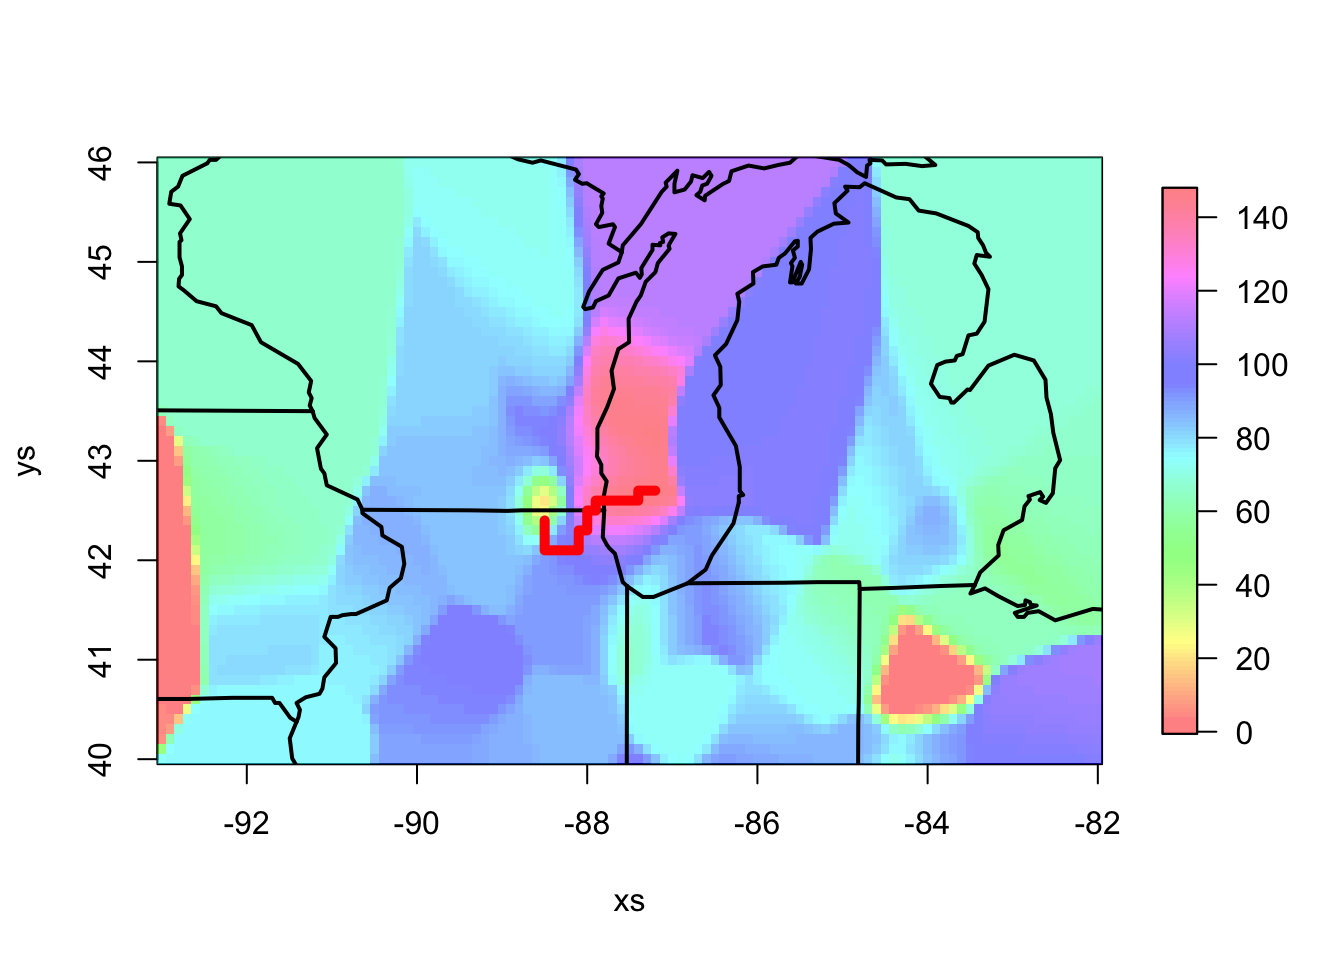
\includegraphics{hw1_files/figure-latex/unnamed-chunk-16-1.pdf}

\subsubsection{Comment:}\label{comment-2}

Our model for linear regression is: \(Y = X*\beta + \epsilon\). The
normality assumption holds, but the residue seems not to be independent
of X. Also, the R-squared is only around 25\%, meaning our model does
not account for much variance in data. p-value suggests that we should
reject the null hypothesis that the selected variables are not
correlated with counts.

\subsection{(b)}\label{b-2}

First, summarize the data by mean hourly counts

\begin{Shaded}
\begin{Highlighting}[]
\NormalTok{varnames =}\StringTok{ }\KeywordTok{dimnames}\NormalTok{(train)[[}\DecValTok{2}\NormalTok{]]}
\NormalTok{ids =}\StringTok{ }\NormalTok{varnames[varnames }\OperatorTok{!=}\StringTok{ "transformed_count"}\NormalTok{]}

\NormalTok{## melt data}
\NormalTok{val_mlt =}\StringTok{ }\KeywordTok{melt}\NormalTok{(val,}\DataTypeTok{id =}\NormalTok{ ids)}
\NormalTok{train_mlt =}\StringTok{ }\KeywordTok{melt}\NormalTok{(train,}\DataTypeTok{id =}\NormalTok{ ids)}

\NormalTok{train_mlt}\OperatorTok{$}\NormalTok{value =}\StringTok{ }\KeywordTok{as.numeric}\NormalTok{(train_mlt}\OperatorTok{$}\NormalTok{value)}
\NormalTok{train_hourmean =}\StringTok{ }\KeywordTok{cast}\NormalTok{(train_mlt,daylabel}\OperatorTok{~}\NormalTok{variable,mean)}

\KeywordTok{attach}\NormalTok{(train_hourmean)}
\KeywordTok{plot}\NormalTok{(daylabel,transformed_count)}
\end{Highlighting}
\end{Shaded}

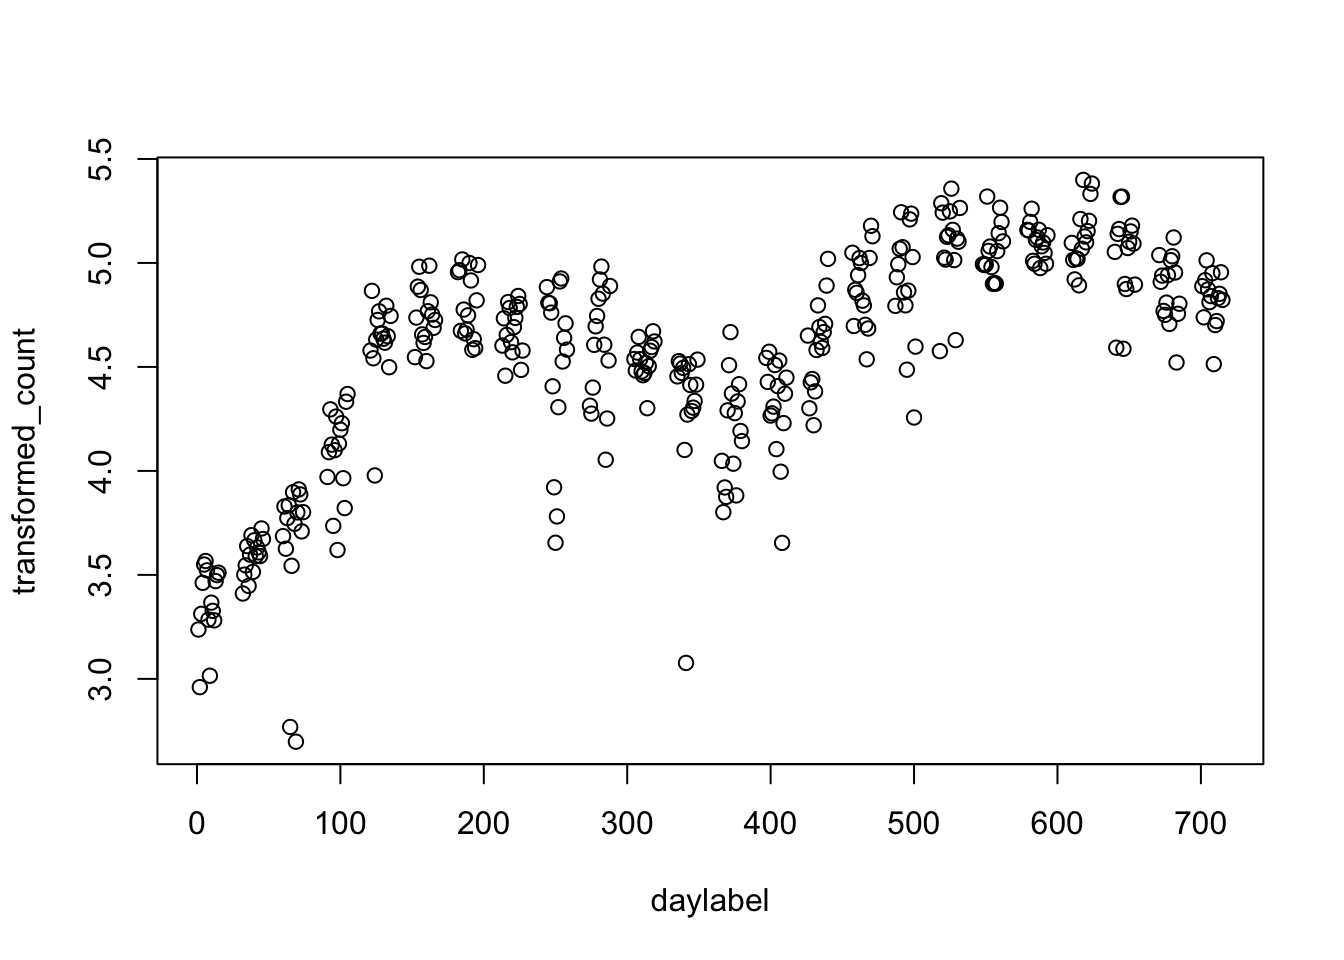
\includegraphics{hw1_files/figure-latex/unnamed-chunk-17-1.pdf}

\begin{Shaded}
\begin{Highlighting}[]
\KeywordTok{attach}\NormalTok{(train_hourmean)}
\end{Highlighting}
\end{Shaded}

\begin{verbatim}
## The following objects are masked from train_hourmean (pos = 3):
## 
##     daylabel, transformed_count
\end{verbatim}

\begin{Shaded}
\begin{Highlighting}[]
\NormalTok{locfitmodel_hourmean_train =}\StringTok{ }\KeywordTok{locfit}\NormalTok{(transformed_count}\OperatorTok{~}\NormalTok{daylabel)}
\NormalTok{predict_hourmean_train =}\StringTok{ }\KeywordTok{predict}\NormalTok{(locfitmodel_hourmean_train,daylabel)}
\KeywordTok{plot}\NormalTok{(daylabel,predict_hourmean_train)}
\end{Highlighting}
\end{Shaded}

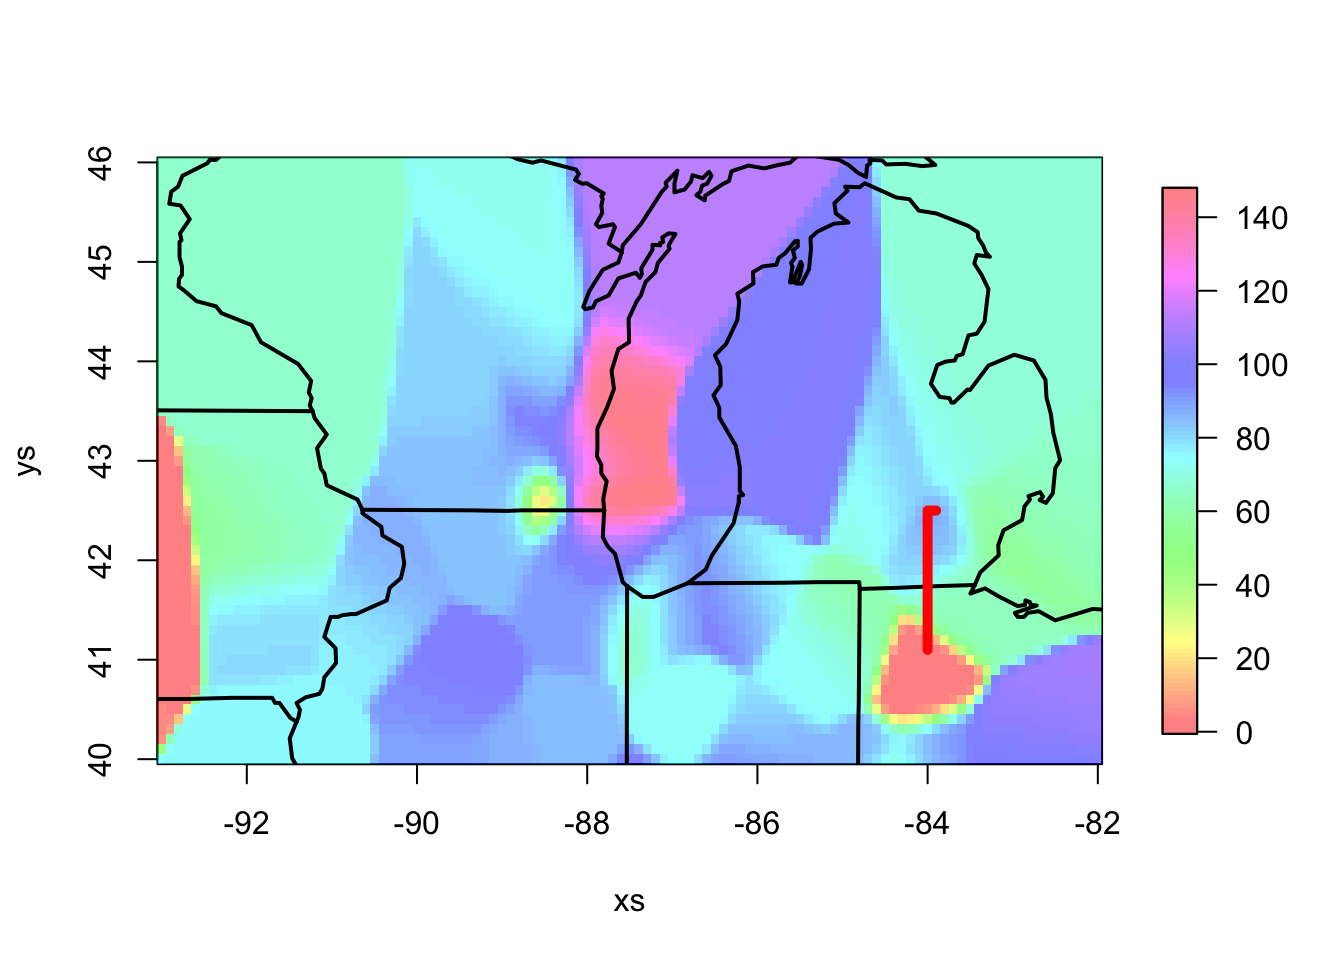
\includegraphics{hw1_files/figure-latex/unnamed-chunk-18-1.pdf}

\begin{Shaded}
\begin{Highlighting}[]
\NormalTok{train_hourmean_trend =}\StringTok{ }\NormalTok{train_hourmean}
\NormalTok{train_hourmean_trend}\OperatorTok{$}\NormalTok{transformed_count =}\StringTok{ }\NormalTok{predict_hourmean_train}

\NormalTok{train_hourmean_residue =}\StringTok{ }\NormalTok{train_hourmean}
\NormalTok{train_hourmean_residue}\OperatorTok{$}\NormalTok{transformed_count =}\StringTok{ }\KeywordTok{residuals}\NormalTok{(locfitmodel_hourmean_train)}
\KeywordTok{detach}\NormalTok{(train_hourmean)}
\end{Highlighting}
\end{Shaded}

\begin{Shaded}
\begin{Highlighting}[]
\NormalTok{u_daylabels =}\StringTok{ }\KeywordTok{unique}\NormalTok{(train_mlt}\OperatorTok{$}\NormalTok{daylabel)}

\NormalTok{## get residue as new response}
\NormalTok{train_residue =}\StringTok{ }\NormalTok{train}

\ControlFlowTok{for}\NormalTok{(i }\ControlFlowTok{in} \DecValTok{1}\OperatorTok{:}\KeywordTok{length}\NormalTok{(u_daylabels))\{}
\NormalTok{  train_residue[train_residue}\OperatorTok{$}\NormalTok{daylabel }\OperatorTok{==}\StringTok{ }\NormalTok{u_daylabels[i],}\StringTok{"transformed_count"}\NormalTok{] =}\StringTok{  }\NormalTok{train_residue[train_residue}\OperatorTok{$}\NormalTok{daylabel }\OperatorTok{==}\StringTok{ }\NormalTok{u_daylabels[i],}\StringTok{"transformed_count"}\NormalTok{] }\OperatorTok{-}\StringTok{ }\NormalTok{train_hourmean_trend[train_hourmean_trend}\OperatorTok{$}\NormalTok{daylabel }\OperatorTok{==}\StringTok{ }\NormalTok{u_daylabels[i],}\StringTok{"transformed_count"}\NormalTok{]}
\NormalTok{\}}

\CommentTok{# SmoothedLinearMD = lm(transformed_count ~ hour+workingday+weather+atemp+humidity+windspeed, data = train_residue)}
\NormalTok{SmoothedLinearMD =}\StringTok{ }\KeywordTok{lm}\NormalTok{(transformed_count }\OperatorTok{~}\StringTok{ }\NormalTok{workingday}\OperatorTok{*}\NormalTok{hour }\OperatorTok{+}\StringTok{ }\NormalTok{season }\OperatorTok{+}\NormalTok{atemp}\OperatorTok{+}\NormalTok{humidity}\OperatorTok{+}\NormalTok{windspeed, }\DataTypeTok{data =}\NormalTok{ train_residue)}





\NormalTok{## training loss}
\NormalTok{LlrLm_train =}\StringTok{ }\KeywordTok{predict}\NormalTok{(SmoothedLinearMD,train) }\OperatorTok{+}\StringTok{ }\KeywordTok{predict}\NormalTok{(locfitmodel_hourmean_train, train}\OperatorTok{$}\NormalTok{daylabel)}
\KeywordTok{print}\NormalTok{(}\KeywordTok{paste0}\NormalTok{(}\StringTok{"training loss: "}\NormalTok{,}\KeywordTok{RMSLE_log}\NormalTok{(LlrLm_train, train}\OperatorTok{$}\NormalTok{transformed_count)))}
\end{Highlighting}
\end{Shaded}

\begin{verbatim}
## [1] "training loss: 0.388239681587841"
\end{verbatim}

\begin{Shaded}
\begin{Highlighting}[]
\NormalTok{## validation loss}
\NormalTok{LlrLm_val =}\StringTok{ }\KeywordTok{predict}\NormalTok{(SmoothedLinearMD,val) }\OperatorTok{+}\StringTok{ }\KeywordTok{predict}\NormalTok{(locfitmodel_hourmean_train, val}\OperatorTok{$}\NormalTok{daylabel)}
\KeywordTok{print}\NormalTok{(}\KeywordTok{paste0}\NormalTok{(}\StringTok{"validation loss: "}\NormalTok{,}\KeywordTok{RMSLE_log}\NormalTok{(LlrLm_val, val}\OperatorTok{$}\NormalTok{transformed_count)))}
\end{Highlighting}
\end{Shaded}

\begin{verbatim}
## [1] "validation loss: 0.381584966746676"
\end{verbatim}

\begin{Shaded}
\begin{Highlighting}[]
\NormalTok{## show how the fit goes }
\KeywordTok{plot}\NormalTok{(val}\OperatorTok{$}\NormalTok{transformed_count[}\DecValTok{1}\OperatorTok{:}\DecValTok{100}\NormalTok{])}
\KeywordTok{lines}\NormalTok{(LlrLm_val[}\DecValTok{1}\OperatorTok{:}\DecValTok{100}\NormalTok{], }\DataTypeTok{col =} \StringTok{"blue"}\NormalTok{)}
\KeywordTok{lines}\NormalTok{(linearPredict_val,}\DataTypeTok{col =} \StringTok{"red"}\NormalTok{)}
\end{Highlighting}
\end{Shaded}

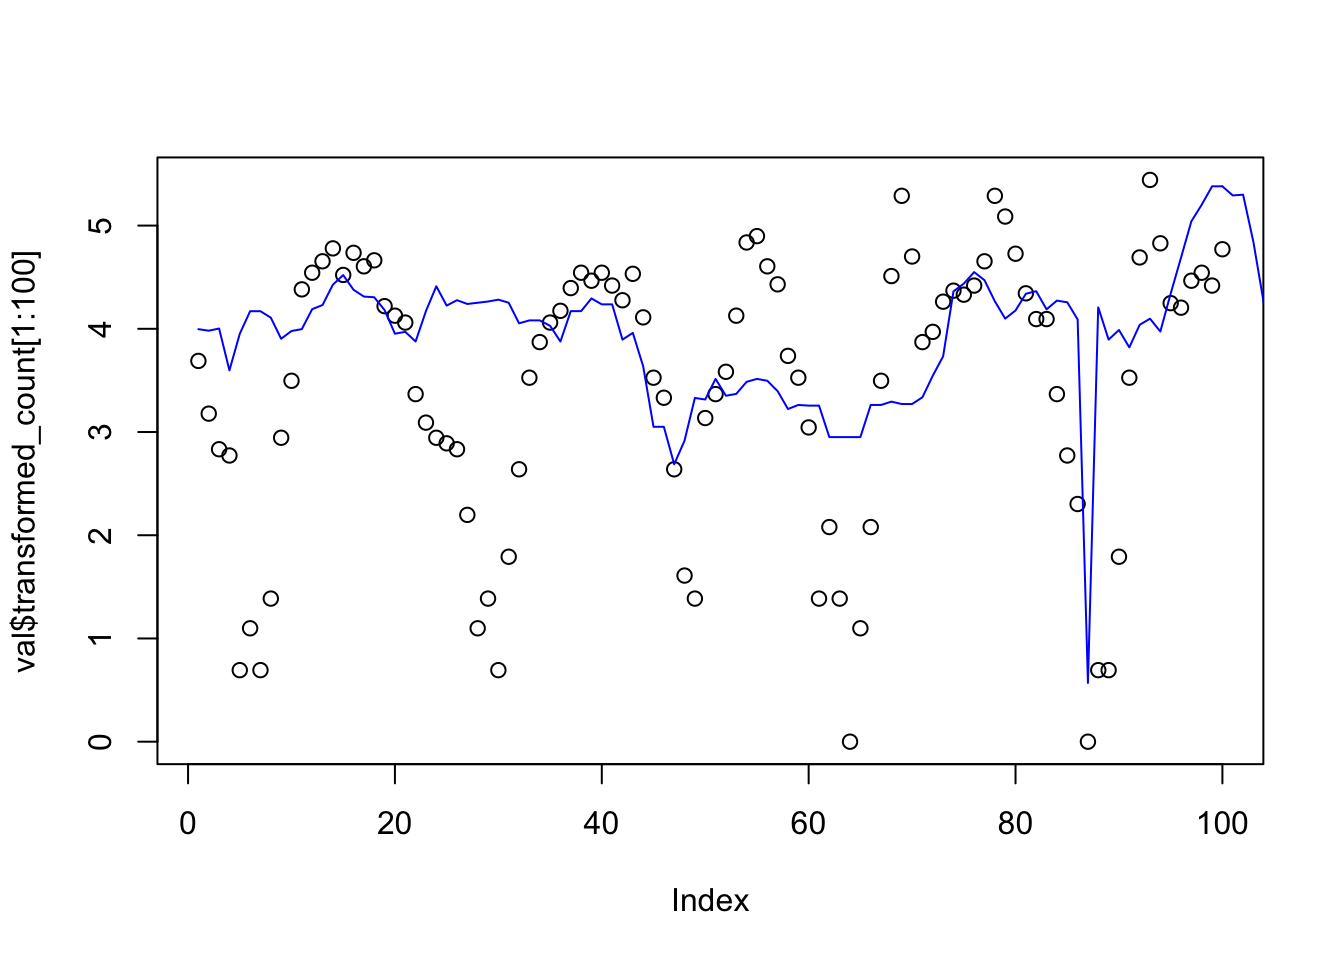
\includegraphics{hw1_files/figure-latex/unnamed-chunk-19-1.pdf}

\subsection{(c) Using additive model}\label{c-using-additive-model}

\begin{Shaded}
\begin{Highlighting}[]
\NormalTok{gamMD <-}\StringTok{ }\KeywordTok{gam}\NormalTok{(transformed_count }\OperatorTok{~}\StringTok{ }\NormalTok{daylabel}\OperatorTok{+}\NormalTok{workingday}\OperatorTok{*}\NormalTok{hour}\OperatorTok{+}\NormalTok{atemp}\OperatorTok{*}\NormalTok{season }\OperatorTok{+}\StringTok{ }\NormalTok{humidity}\OperatorTok{+}\NormalTok{workingday}\OperatorTok{+}\NormalTok{holiday}\OperatorTok{*}\NormalTok{weather, }\DataTypeTok{data =}\NormalTok{ train_residue)}
\CommentTok{#gamMD <- gam(transformed_count ~ daylabel+workingday+hour+workingday*hour + season +atemp+humidity+windspeed, data = train_residue)}

\NormalTok{## training loss}
\NormalTok{GamLm_train =}\StringTok{ }\KeywordTok{predict}\NormalTok{(gamMD,train) }\OperatorTok{+}\StringTok{ }\KeywordTok{predict}\NormalTok{(locfitmodel_hourmean_train, train}\OperatorTok{$}\NormalTok{daylabel)}
\KeywordTok{print}\NormalTok{(}\KeywordTok{paste0}\NormalTok{(}\StringTok{"training loss: "}\NormalTok{,}\KeywordTok{RMSLE_log}\NormalTok{(GamLm_train, train}\OperatorTok{$}\NormalTok{transformed_count)))}
\end{Highlighting}
\end{Shaded}

\begin{verbatim}
## [1] "training loss: 0.360566240953876"
\end{verbatim}

\begin{Shaded}
\begin{Highlighting}[]
\NormalTok{## validation loss}
\NormalTok{GamLm_val =}\StringTok{ }\KeywordTok{predict}\NormalTok{(gamMD,val) }\OperatorTok{+}\StringTok{ }\KeywordTok{predict}\NormalTok{(locfitmodel_hourmean_train, val}\OperatorTok{$}\NormalTok{daylabel)}
\KeywordTok{print}\NormalTok{(}\KeywordTok{paste0}\NormalTok{(}\StringTok{"validation loss: "}\NormalTok{,}\KeywordTok{RMSLE_log}\NormalTok{(GamLm_val, val}\OperatorTok{$}\NormalTok{transformed_count)))}
\end{Highlighting}
\end{Shaded}

\begin{verbatim}
## [1] "validation loss: 0.35068072795119"
\end{verbatim}

\begin{Shaded}
\begin{Highlighting}[]
\NormalTok{## show how the fit goes }
\KeywordTok{plot}\NormalTok{(val}\OperatorTok{$}\NormalTok{transformed_count[}\DecValTok{1}\OperatorTok{:}\DecValTok{100}\NormalTok{])}
\KeywordTok{lines}\NormalTok{(GamLm_val[}\DecValTok{1}\OperatorTok{:}\DecValTok{100}\NormalTok{], }\DataTypeTok{col =} \StringTok{"green"}\NormalTok{)}
\KeywordTok{lines}\NormalTok{(LlrLm_val[}\DecValTok{1}\OperatorTok{:}\DecValTok{100}\NormalTok{], }\DataTypeTok{col =} \StringTok{"blue"}\NormalTok{)}
\KeywordTok{lines}\NormalTok{(linearPredict_val,}\DataTypeTok{col =} \StringTok{"red"}\NormalTok{)}
\end{Highlighting}
\end{Shaded}

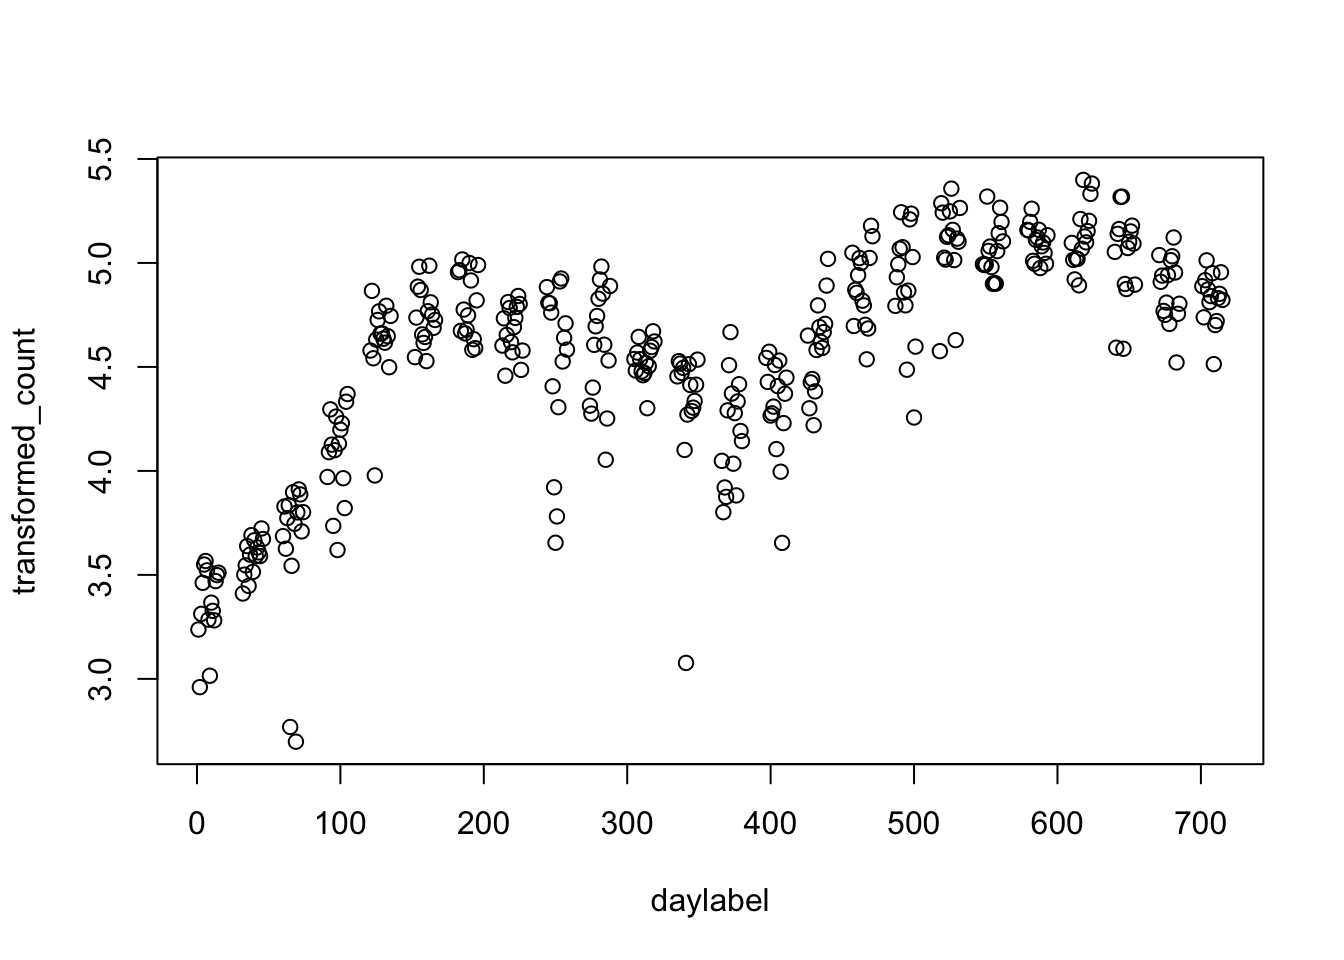
\includegraphics{hw1_files/figure-latex/unnamed-chunk-20-1.pdf}

\subsection{Comment:}\label{comment-3}

I got the best prediction from part (c). Though gam can lift my the
model performance a little, feature selection is perhaps more important.
Before adding the interaction term for workingday*hour, my best loss is
around 1, much worse than the simplist linear model used here.

\begin{Shaded}
\begin{Highlighting}[]
\NormalTok{## prediction on test}
\NormalTok{GamLm_test =}\StringTok{ }\KeywordTok{predict}\NormalTok{(gamMD,test) }\OperatorTok{+}\StringTok{ }\KeywordTok{predict}\NormalTok{(locfitmodel_hourmean_train, test}\OperatorTok{$}\NormalTok{daylabel)}
\KeywordTok{write.table}\NormalTok{(}\KeywordTok{as.numeric}\NormalTok{(GamLm_test), }\StringTok{"../data/assn1-wangzh.txt"}\NormalTok{, }\DataTypeTok{row.names =} \OtherTok{FALSE}\NormalTok{, }\DataTypeTok{col.names=}\OtherTok{FALSE}\NormalTok{, }\DataTypeTok{sep =} \StringTok{"}\CharTok{\textbackslash{}n}\StringTok{"}\NormalTok{)}
\end{Highlighting}
\end{Shaded}


\end{document}
